\documentclass[conference]{IEEEtran}
\IEEEoverridecommandlockouts
\usepackage{cite}
\usepackage{amsmath,amssymb,amsfonts,amsthm}
\usepackage{algorithmic}
\usepackage{graphicx}
\usepackage{textcomp}
\usepackage{xcolor}
\usepackage{url}
\usepackage{hyperref}
\usepackage{lipsum}
\usepackage{bm}
\usepackage{array}
\usepackage{cite}
\usepackage{listings}
\usepackage{gensymb}
\usepackage[justification=centering]{caption}
\def\BibTeX{{\rm B\kern-.05em{\sc i\kern-.025em b}\kern-.08em
    T\kern-.1667em\lower.7ex\hbox{E}\kern-.125emX}}
    
    \definecolor{dkgreen}{rgb}{0,0.6,0}
\definecolor{gray}{rgb}{0.5,0.5,0.5}
\definecolor{mauve}{rgb}{0.58,0,0.82}

\lstset{frame=tb,
  language=R,
  aboveskip=3mm,
  belowskip=3mm,
  showstringspaces=false,
  columns=flexible,
  basicstyle={\small\ttfamily},
  numbers=none,
  numberstyle=\tiny\color{gray},
  keywordstyle=\color{blue},
  commentstyle=\color{dkgreen},
  stringstyle=\color{mauve},
  breaklines=true,
  breakatwhitespace=true,
  tabsize=3
}
    
\begin{document}

\title{Practical Software Reliability Modeling and Application: A Case Study
\thanks{This work is supported by NASA under contract number: }
}



\author{\IEEEauthorblockN{Vidhyashree Nagaraju, Shekar, Niti, and Lance Fiondella}
\IEEEauthorblockA{Department of Electrical and Computer Engineering\\
University of Massachusetts, Dartmouth, MA, 02747 USA\\
Email: \{vnagaraju,lfiondella\}@umassd.edu}
\and
\IEEEauthorblockN{Ying Shi}
\IEEEauthorblockA{Goddard Space Flight Center\\
National Aeronautics and Space Administration\\
Email: @}}

\maketitle

\begin{abstract}
This paper demonstrates the utility of a script to automatically apply a free and open source software failure and reliability assessment tool. The script generates a pdf report, eliminating the need to work with the user interface of the tool to manually assess the data and report. The reports can be used to summarize progress to both technical and non-technical leadership. Simplifying the assessment and reporting may encourage the software and reliability practitioners to apply the models and make decisions about the process.
\end{abstract}

\begin{IEEEkeywords}
Software reliability, software reliability growth model, R statistical programming language, GitHub, Software Failure and Reliability Assessment Tool, open source
\end{IEEEkeywords}


\section{Introduction}\label{sec:Intro}
Software reliability growth models (SRGM)~\cite{BookHoSRE} are extremely useful in making decisions about software development by characterizing failure data collected during testing. Some of the predictions featured by SRGM include the remaining number of failures, failure intensities, mean time to failures, release time, as well as overall software reliability. However, practitioners may be reluctant to apply these models due to a lack of either the knowledge of the underlying mathematics or the time to develop expertise and implement models in their work. Therefore, several computer-aided software reliability tools~\cite{trSMERFS,inProcISSRE2013_100,lyu1992casre} have been developed.

Previous computer-aided tools to apply software reliability methods include: Emerald~\cite{1996hudepohlemerald}, SRMP (Software Reliability Modeling Programs)~\cite{1988SRMP}, the AT\&T SRE Toolkit~\cite{1990ATT}, SoRel~\cite{1993kanounsorel}, SMERFS (Statistical Modeling and Estimation of Reliability Functions for Software)~\cite{trSMERFS}, and CASRE (Computer Aided Software Reliability Estimation)~\cite{lyu1992casre}, Robust~\cite{1995lirobust}, SREPT~\cite{2000ramanisrept}, CARATS~\cite{2011huangestimation}, SRATS~\cite{inProcISSRE2013_100}, and M-SRAT~\cite{2015shibatam}. Most of these tools are mostly spreadsheet based~\cite{inProcISSRE2013_100} or close source in nature. This inhibits the capability to integrate the existing tools into software testing work flows and update the tools with recent changes in the software reliability research. To overcome the limitation of existing tools, an open source Software Failure and Reliability Assessment Tool (SFRAT)~\cite{cFio53} is developed with a flexible architecture to accommodate individual researchers models as well as methods.

In this paper, we present a script to automatically apply an open source SFRAT and generate report. This script eliminates the need to work with the graphical user interface to manually prepare the report, thus conserving time. The script can be configured to produce custom reports; for example, the user can opt to include explanations of each result in the report. The script generates a pdf to visually assess the data and to ease the reporting process. The reports can then be used to summarize and visualize project status to both technical and non-technical leadership.

The remainder of the paper is organized as follows: Section~\ref{sec:SFRAT} provides a brief overview of the SFRAT user interface and Section~\ref{sec:Script} provides a detailed discussion of the script to generate the report automatically. Section~\ref{sec:Ex} demonstrates the use of the script through a real data, while Section~\ref{sec:Concl} provides conclusion and directions for future research.


\section{Software Failure and Reliability Assessment Tool (SFRAT)}\label{sec:SFRAT}
The Software Failure and Reliability Assessment Tool is a free and open source tool developed to promote quantitative assessment of software reliability as well as improved communications of such assessments. SFRAT is an application that estimates and predicts the reliability of a software system during test and operation. Some of the questions that the tool answers about a system undergoing test are:
\begin{itemize}
\item {Is the software reliable enough to release?}
\item {How long will it be before a specified goal is reached?}
\item {What will be the consequences if testing resources are insufficient?}
\end{itemize}

SFRAT is implemented in the R statistical programming language~\cite{}, an open source environment for statistical computing and graphics that can be used on computers running Windows, OSX, or Linux, with the user interface implemented using the R Shiny library~\cite{}. The code is accessible on GitHub at \textit{https://github.com/LanceFiondella/srt.core}, which after downloading can be ran using RStudio or any other R environment. In doing so, an organization can easily perform information assurance of the code prior to use on sensitive failure data. For complete details, the reader is referred to \textit{http://sasdlc.org/lab/projects/srt.html}.
%re-word sentence 3 below
The architecture of the SFRAT combines the use of existing software reliability models into a single tool, enabling more systematic comparison of models than previously possible. Presently, data formats supported consist of inter failure time, failure time, and failure count. Functionality includes two trend tests for reliability growth, two failure rate~\cite{BookHoSRE}, Jelinski-Moranda and geometric, and three failure counting models, Goel-Okumoto~\cite{goel1985software}, delayed S-shaped~\cite{artTR1986_19}, and Weibull~\cite{artNHPPsurvey} models as well as two measures of goodness of fit. Also implemented are methods to predict time to reach a desired reliability as well as detecting a number of future failures. The free and open source nature of the tool architecture enables additional models and goodness of fit measures to be later implemented. In this regard, the tool is intended to serve as a shared environment for collaboration among researchers and practitioners.

SFRAT can be accessed by downloading the source code from GitHub and run using an R environment (e.g. RStudio), or through the web instance. Once the application is launched, the initial SFRAT screen is shown as seen in Figure~\ref{fig_DefaultView}.
\begin{figure}[!h]
\centering
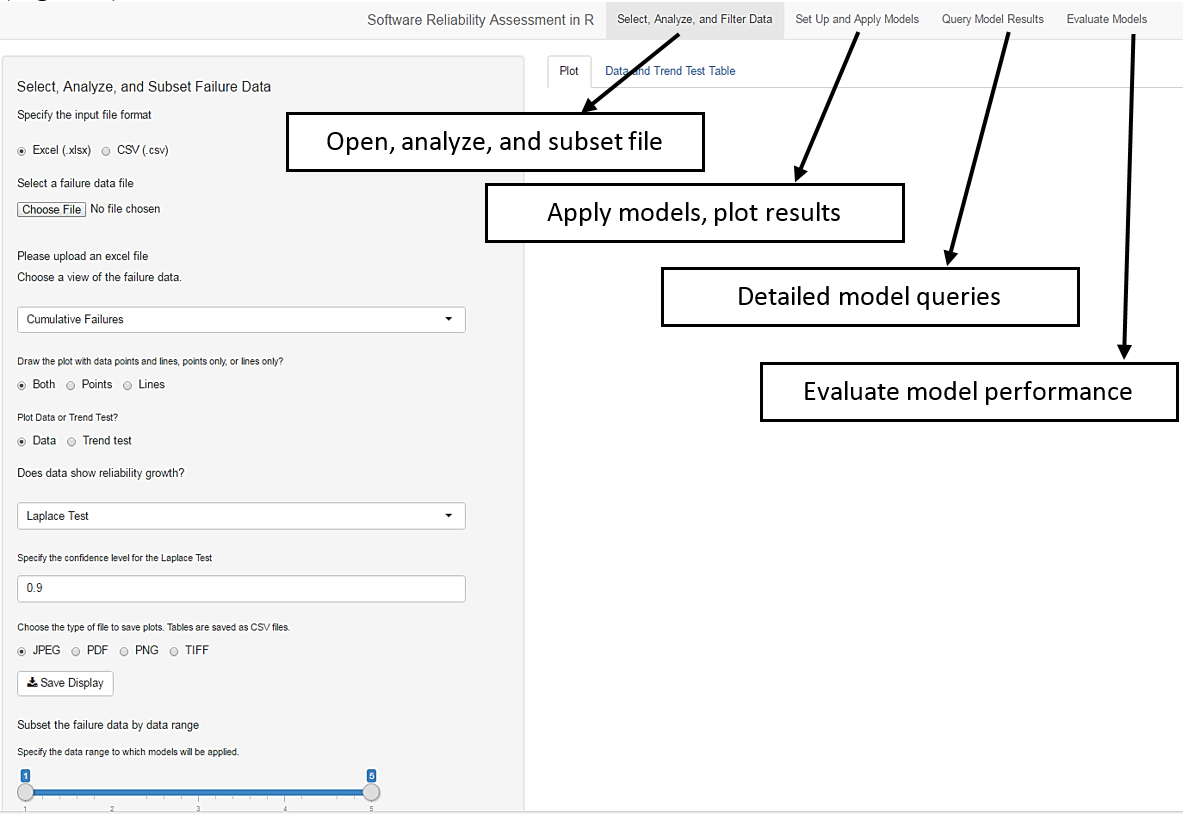
\includegraphics[width=\columnwidth]{Figures/DefaultView}
\caption{Initial View within SFRAT}
\label{fig_DefaultView}
\end{figure}


The SFRAT workflow is divided into four subtasks:
\begin{itemize}
\item{\textbf{Select, Analyze, and Filter Data}: Import failure data history and determine model applicability of its reliability's growth.}
\item{\textbf{Set Up and Apply Models}: View results of one or more reliability models, including reliability growth.}
\item{\textbf{Query Model Results}: Query applied models to answer the following questions:
\begin{itemize}
\item{How many additional failures will occur during a continued period of testing?}
\item{How much time would be required to observe a number of additional failures?}
\item{At what point in testing will a reliability goal be reached?}
\end{itemize}}
\item{\textbf{Evaluate Models}: By model comparison, determine which is most likely to proficiently characterize the data and provide accurate predictions.}
\end{itemize}


\subsection{Tab 1: Select, Analyze, and Filter Data}\label{tab1}
Figure~\ref{fig_Tab1_leftCol} shows the options in the first tab, which includes file selection, data visualization, and trend test analysis. The user can then use the tool by specifying the input file as either an Excel spreadsheet (.xlsx) or a CSV (comma separated value) (.csv) format. The input file must follow the format shown in Figure~\ref{fig_Excel_sys1}, where failure number(FN), interfailure time(IF), and failure time(FT) are indicated.

\begin{figure}[!h]
\centering
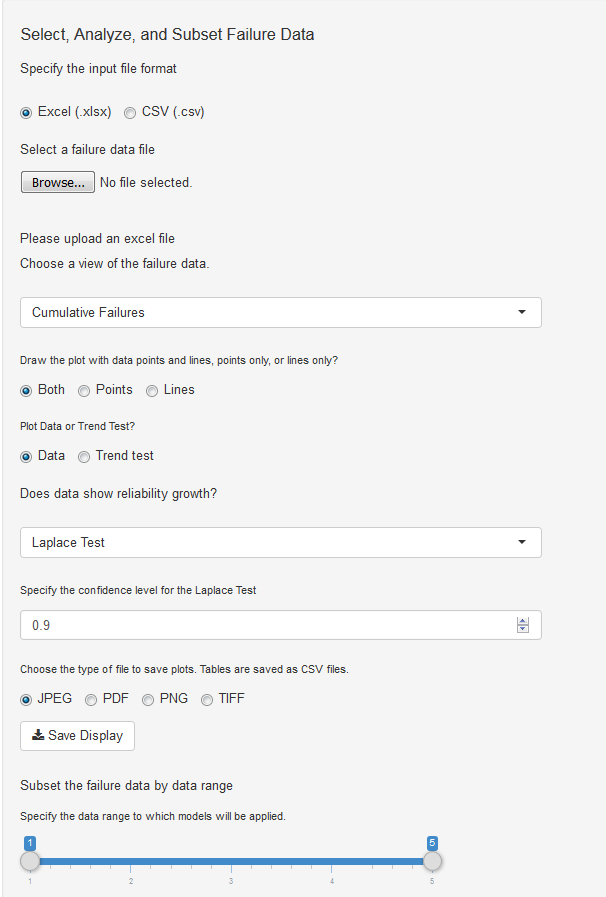
\includegraphics[width=3.4in]{Figures/Fig2}
\caption{Tab one view}
\label{fig_Tab1_leftCol}
\end{figure}

\begin{figure}[!h]
\centering

\includegraphics[width=1.8in]{Figures/sys1excel}
\caption{Example Excel input}
\label{fig_Excel_sys1}
\end{figure}

Clicking on the \textbf{Browse...} button enables the user search for and upload the input data file. The progress bar message ``Upload complete'' will indicate a successful file upload. By default, a plot of the cumulative failures for the uploaded data set is displayed. For example, Figure~\ref{fig_Tab1_CDF} shows the SYS1 data set~\cite{BookHoSRE}.

\begin{figure}[!h]
\centering
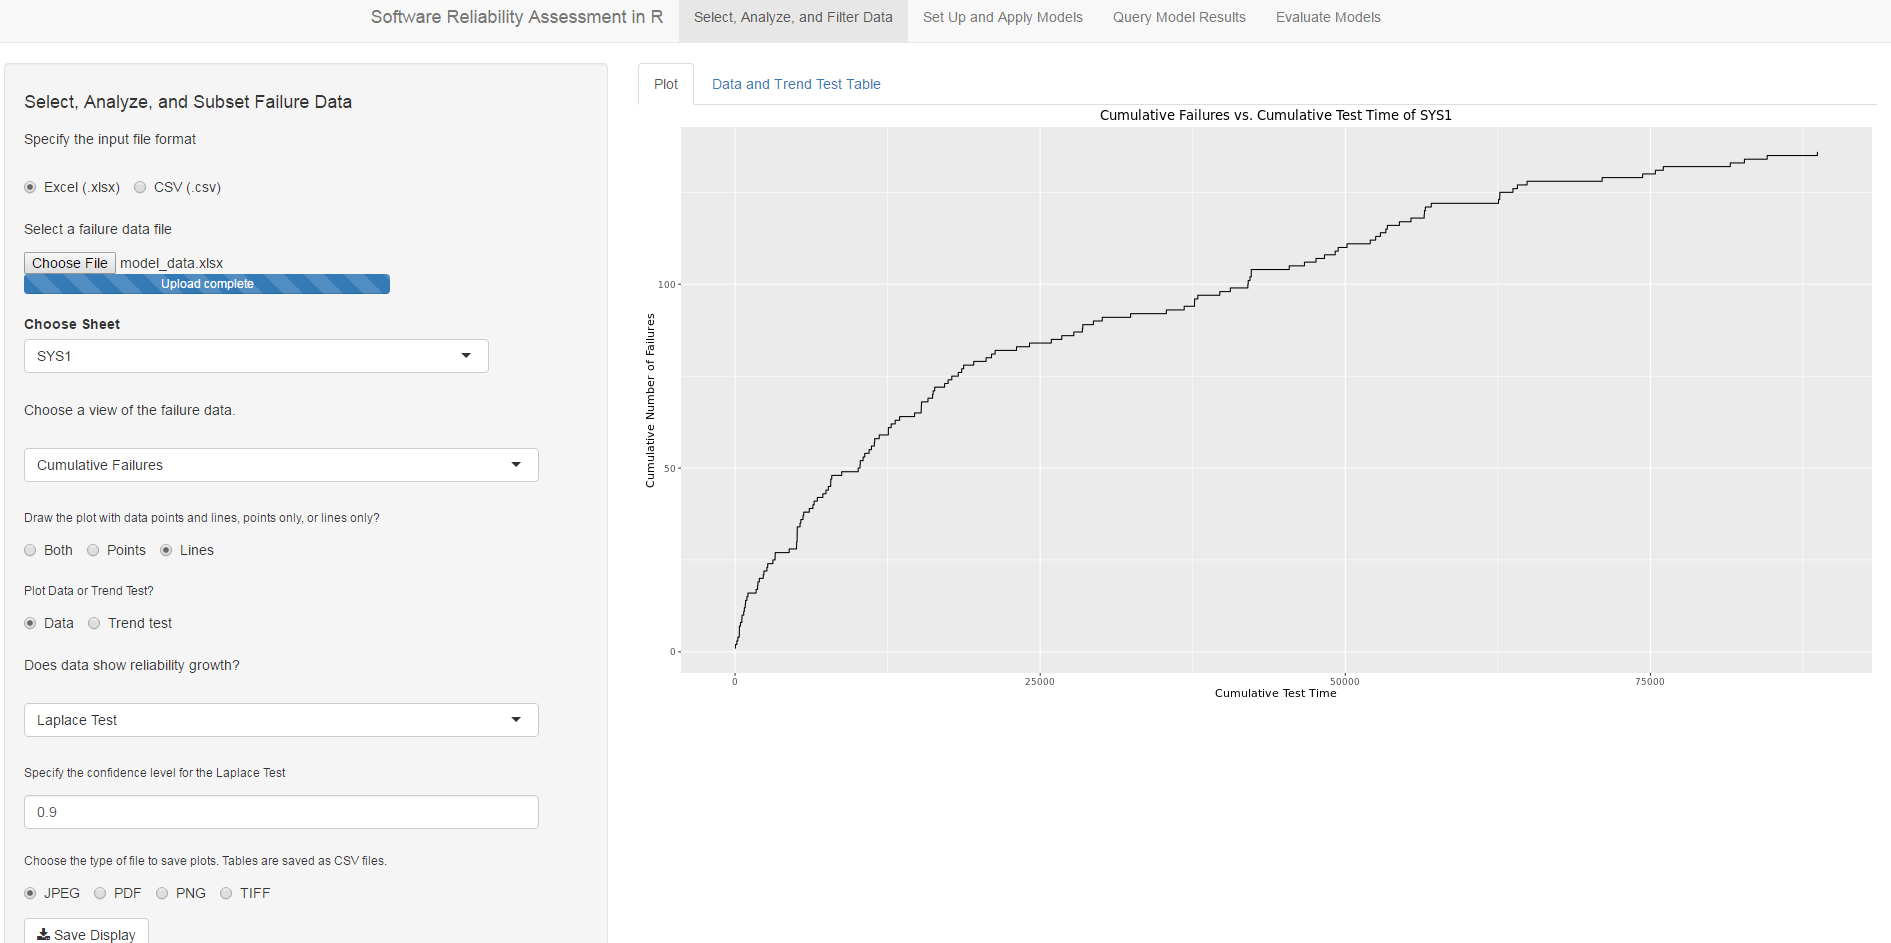
\includegraphics[width=3.4in, height=3in]{Figures/Fig4}
\caption{Tab one view after upload}
\label{fig_Tab1_CDF}
\end{figure}


From a drop-down menu below the progress bar, the user may choose from the provided data sets. CSV files may only contain only one data set, whereas Excel files will contain one data set per sheet. Data sets that do not comply with the input format will not be available in the dropdown menu. Regardless of the input's data format, the tool will provide conversions to failure time, failure count, and inter failure data formats upon upload, allowing for the use of any data model. $31$ data sets were taken from the Handbook of Software Reliability Engineering~\cite{BookHoSRE} and prepared in the file format. Of these, $10$ are failure time data and the remaining $21$ are failure counts. This enables a more comprehensive comparison between models than previously possible. Using the drop-down menu below ``Choose a view of the failure data'', the user may select an alternative data view, including failure intensities and the times between failures. In addition, the option exists to draw plots with either points, lines or both.

Data and Trend test plotting is also possible by use of the radio buttons with the same labels. These trend tests have been placed before model fitting to ensure that the data exhibits reliability growth and is therefore appropriate for software reliability models and predictions. The two tests implemented include the Laplace trend test~\cite{gaudoin1992optimal} as well as a running arithmetic average.

Figure~\ref{fig_Tab1_Laplace} shows the Laplace trend test of the SYS1 data set. The red line seen is a user-specified input, entered into the text box just underneath the Laplace Test drop-down box, as shown in Figure~\ref{fig_Tab1_leftCol}. In this case, the value has been set to $0.9$ or $90\%$. Additional default levels in black include $90$, $95$, $99$, $99.9$, $99.9999$, and $99.999999$. Values below these lines indicate that the data exhibits reliability growth with the specified level of statistical significance and is therefore suitable to apply software reliability models.

\begin{figure}[!h]
\centering
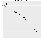
\includegraphics[width=3.4in]{Figures/SRT3}
\caption{Laplace trend test}
\label{fig_Tab1_Laplace}
\end{figure}


Figure~\ref{fig_SRT_RAT} shows the running arithmetic average of the SYS1 data set. Intuitively, if the time between failures increases then the running arithmetic average increases, indicating system reliability is improving. A decreasing running arithmetic average indicates reliability deterioration. Both the Laplace trend test and running arithmetic average suggest the SYS1 data set exhibits reliability growth.

\begin{figure}[!h]
\centering
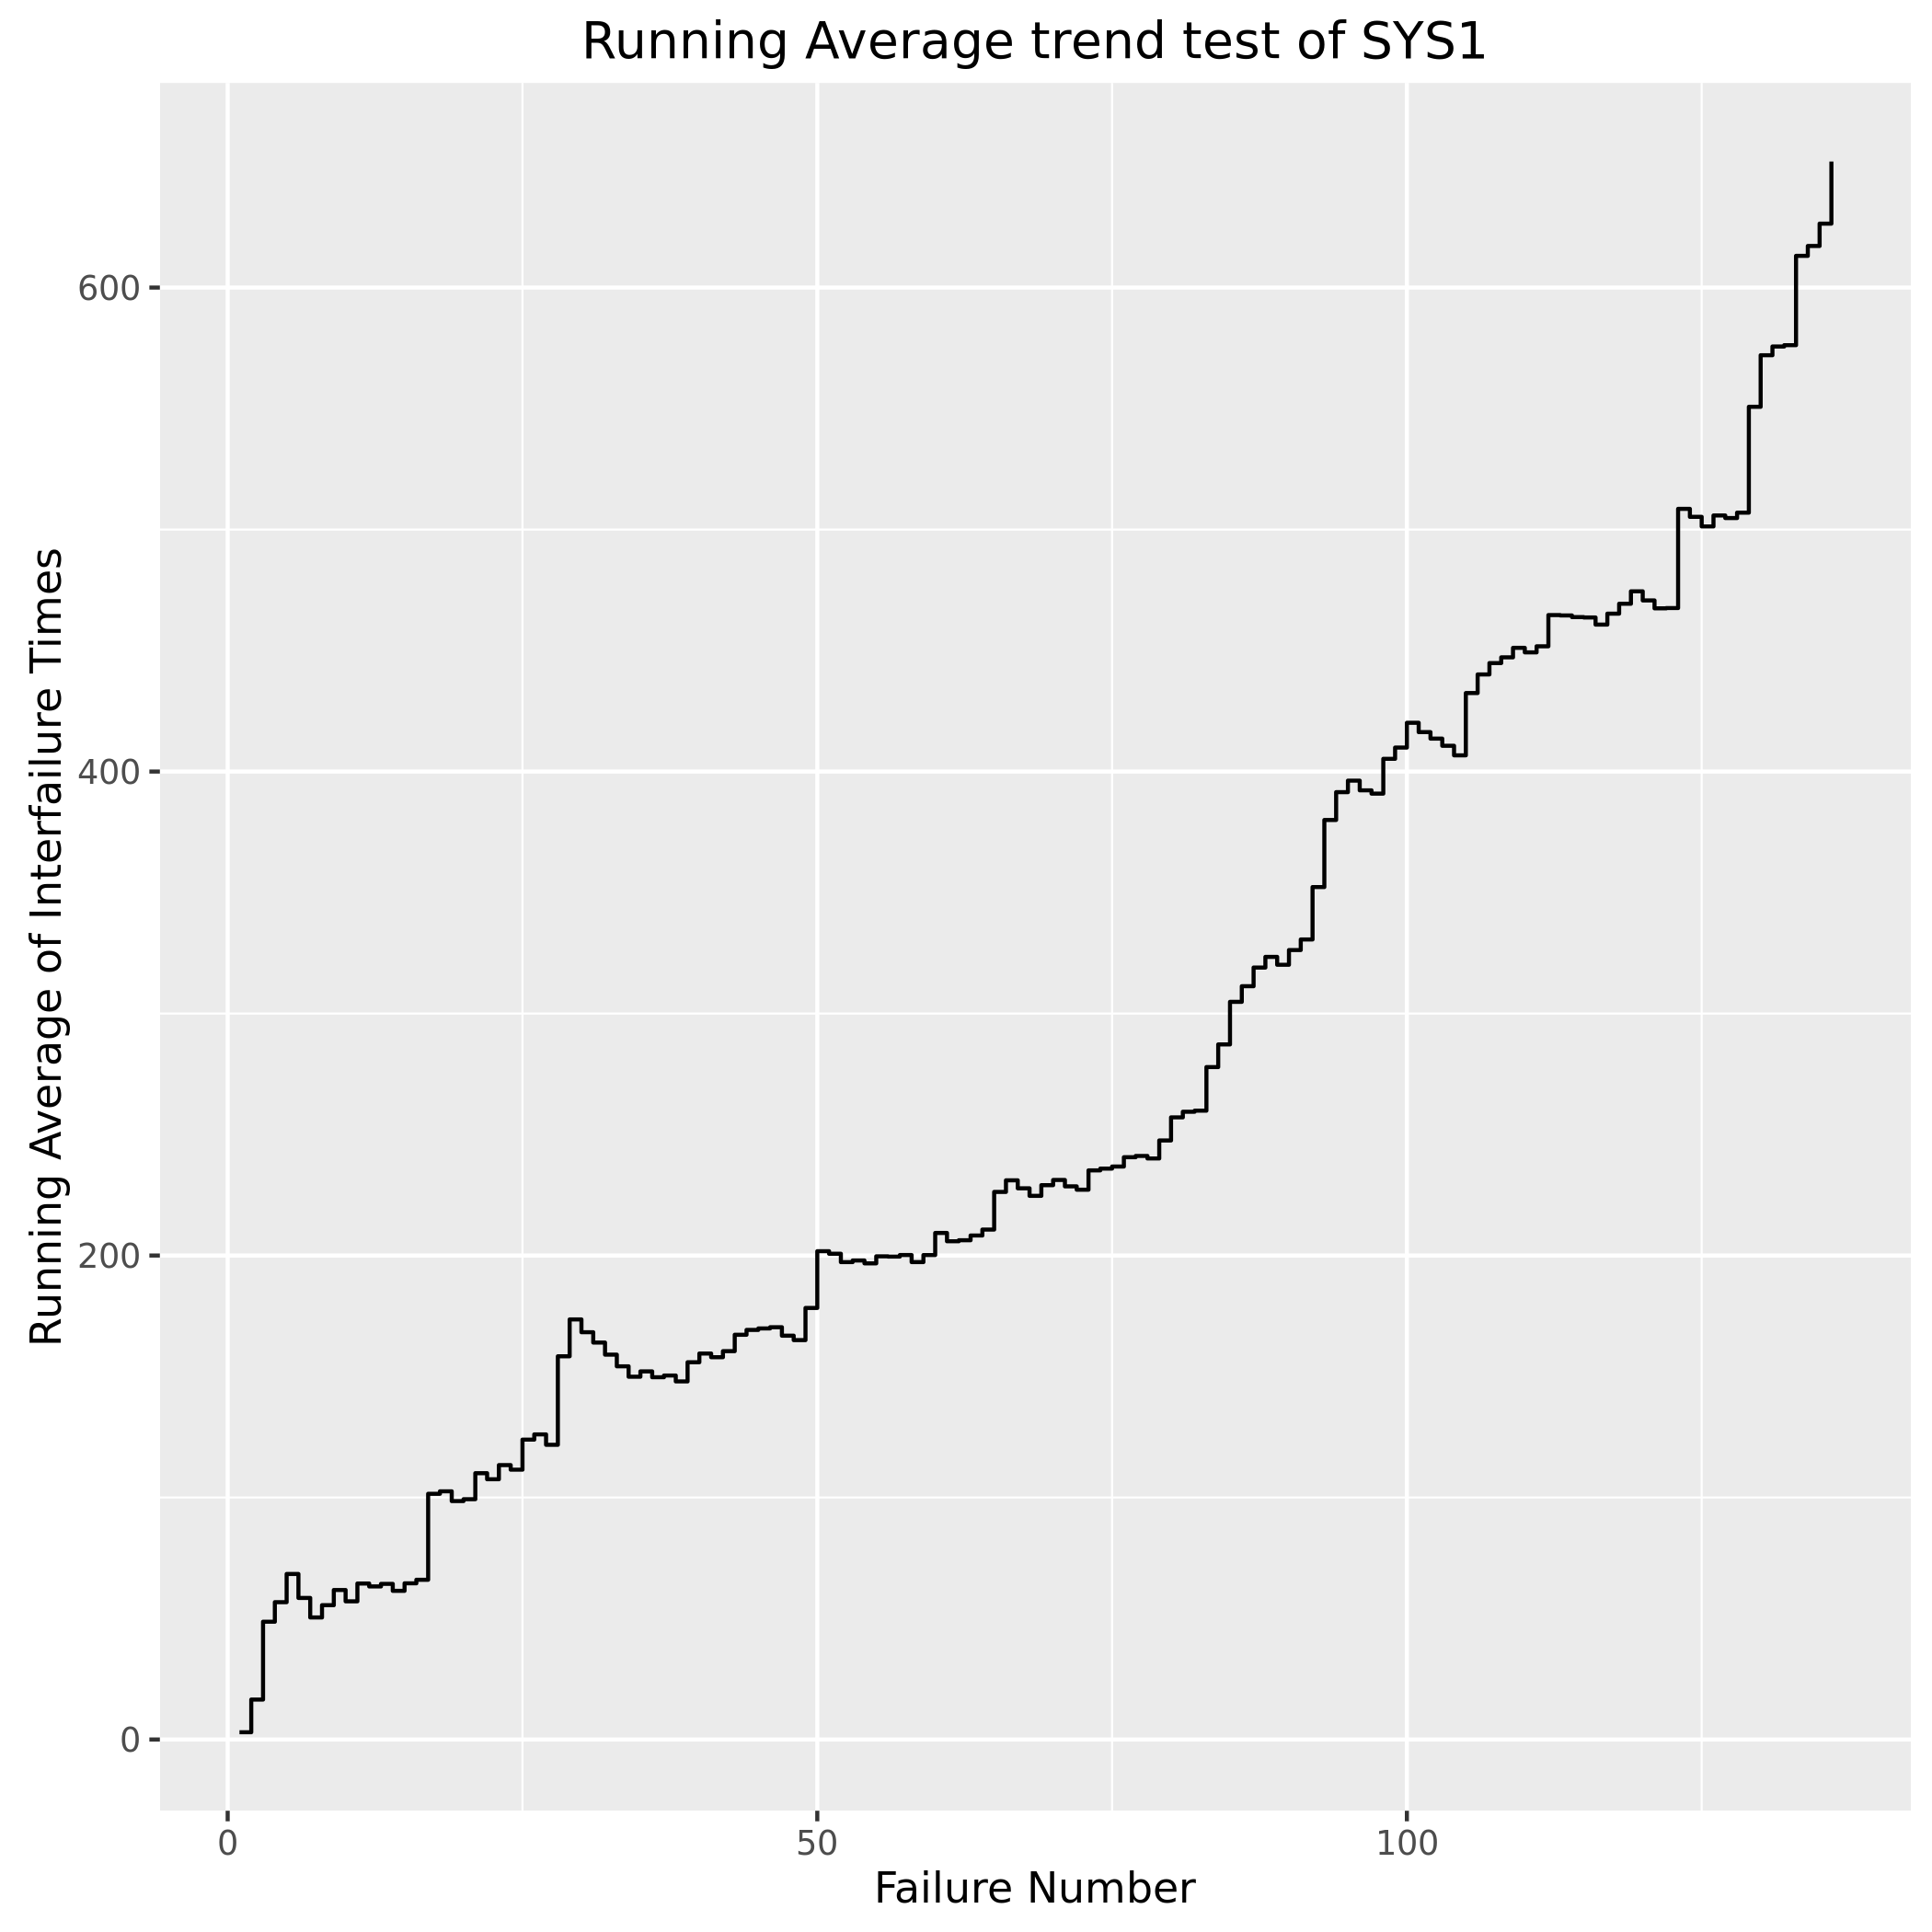
\includegraphics[width=3.4in]{Figures/SRT_RAT}
\caption{Running arithmetic average}
\label{fig_SRT_RAT}
\end{figure}


Figure~\ref{fig:J4Trend} shows the Laplace trend test of the J4 data set which does not experience statistically significant reliability improvement. Thus, it is not appropriate to apply software reliability models to this data set until additional testing is performed that establishes confidence in reliability growth. The slider at the bottom of Figure~\ref{fig_Tab1_leftCol} ranges from $1$ to $n$, where $n$ denotes the number of data points contained in a data set. The sliders allow the user to specify a subset of the data for plotting, model fitting, and prediction. The default is to use all $n$ data points for model fitting.

\begin{figure}[!h]
\centering
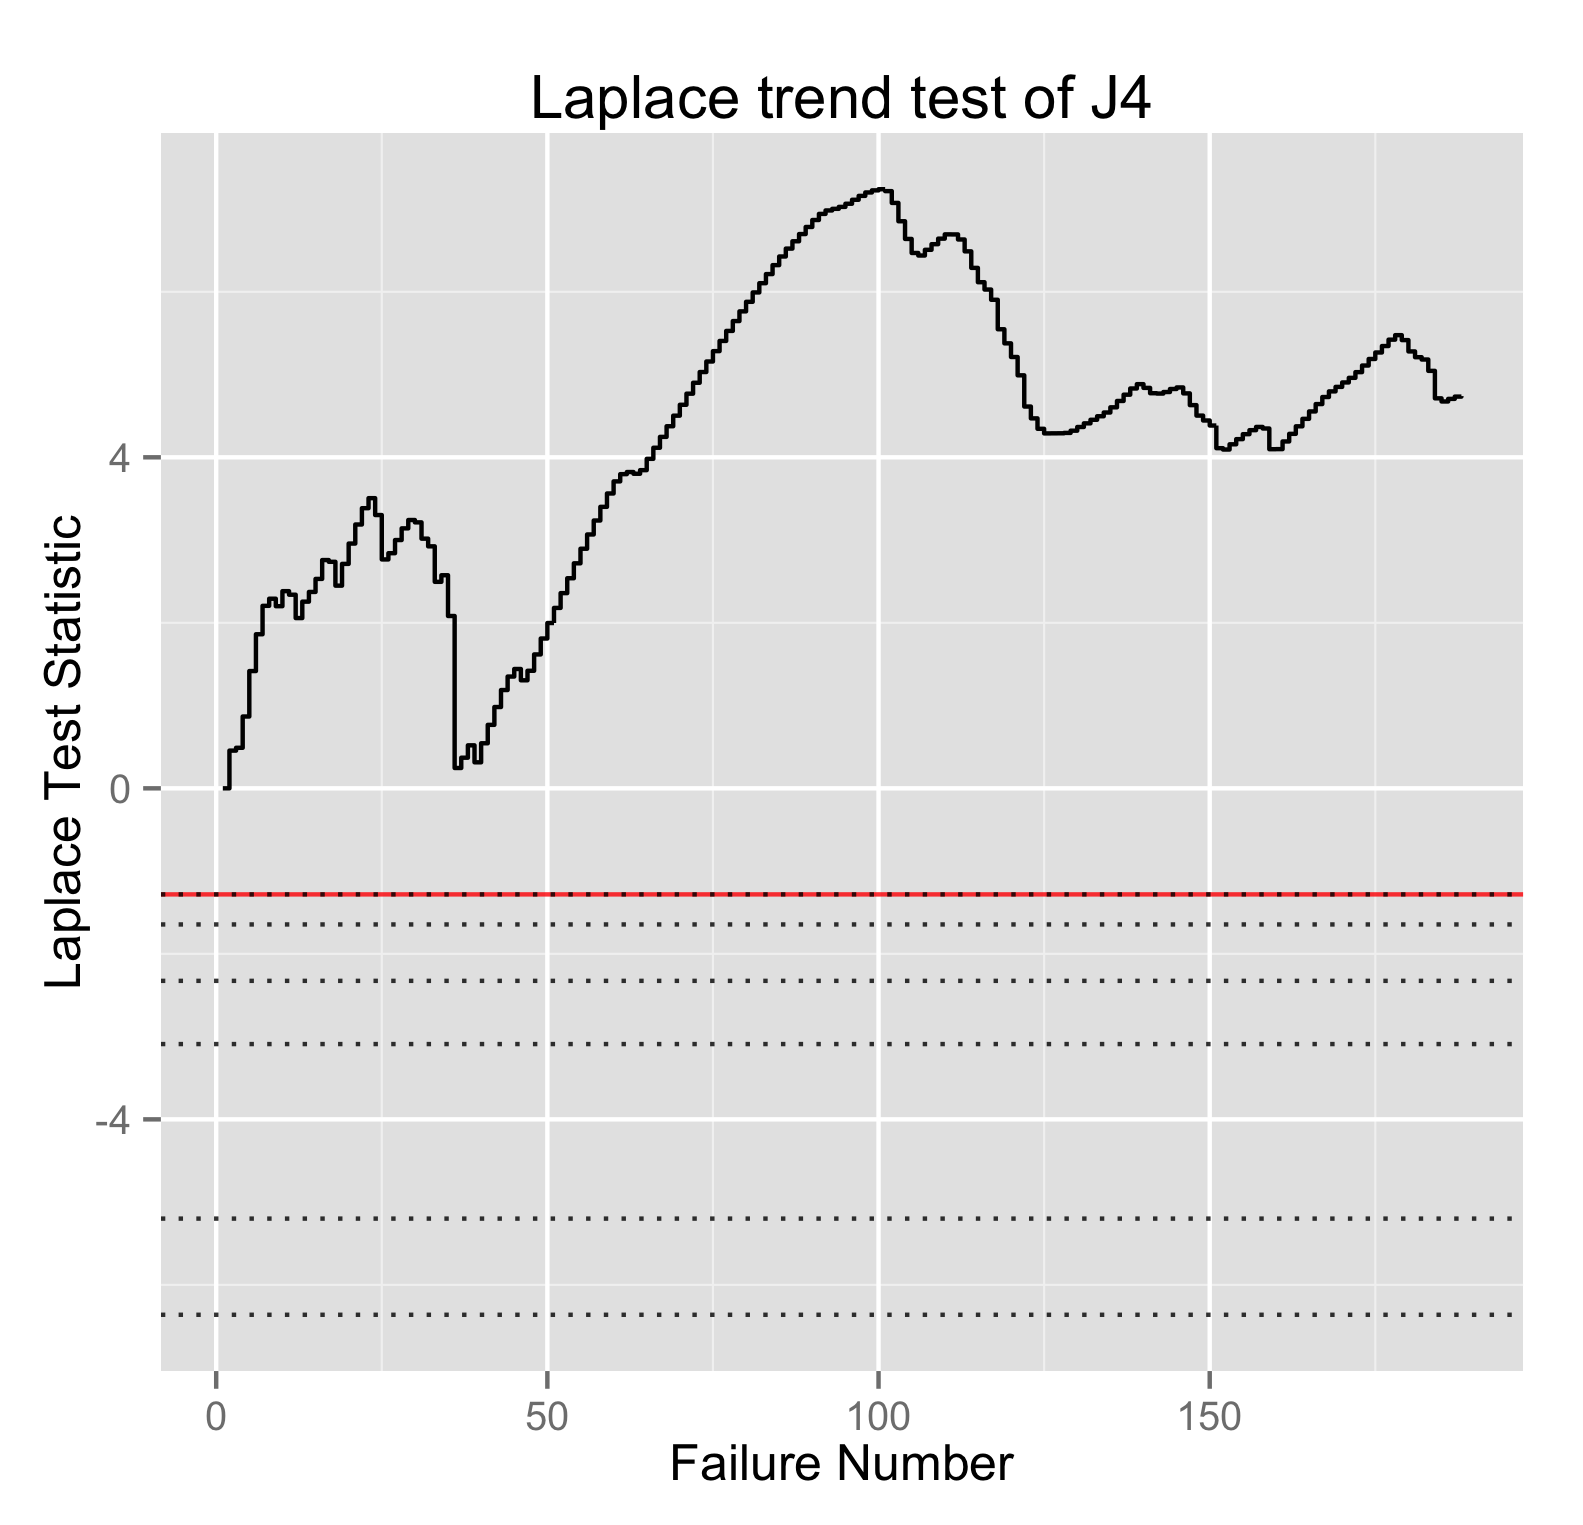
\includegraphics[width=3.4in,height=2in]{Figures/J4_Trend_LP}
\caption{Data set without reliability growth}
\label{fig:J4Trend}
\end{figure}

The user can switch between the \textbf{Plot} and~\textbf{Data and Trend Test Table} in Figure~\ref{fig_Tab1_CDF}. Selecting table view displays the numerical data used to draw the plots in a tabular format similar to Figure~\ref{fig_Excel_sys1}. Selecting a radio button \textbf{.jpeg}, \textbf{.pdf}, \textbf{.png}, and \textbf{.tiff} (Figure~\ref{fig_Tab1_leftCol}) and then clicking \textbf{Save Display} saves a plot in the desired image format, while tables can be saved as csv or pdf. Tabular data can be exported to input into graphing software to include images in reports and research papers.


\subsection{Tab 2: Set up and Apply Models}\label{tab2}
Figure~\ref{fig_Tab2} shows the options available on the second tab where model fitting is performed. The first text box allows the user to ``Specify the number of failures for which the models will make predictions''. Here the number of failures has been set to one for the sake of illustration. The second multi-select box allows the user to identify which models to fit with the data range chosen on Tab one. By default, the tool displays all available models. Clicking the \textbf{Run Selected Models} button executes the algorithms to fit selected model.

\begin{figure}[!h]
\centering%SRT5
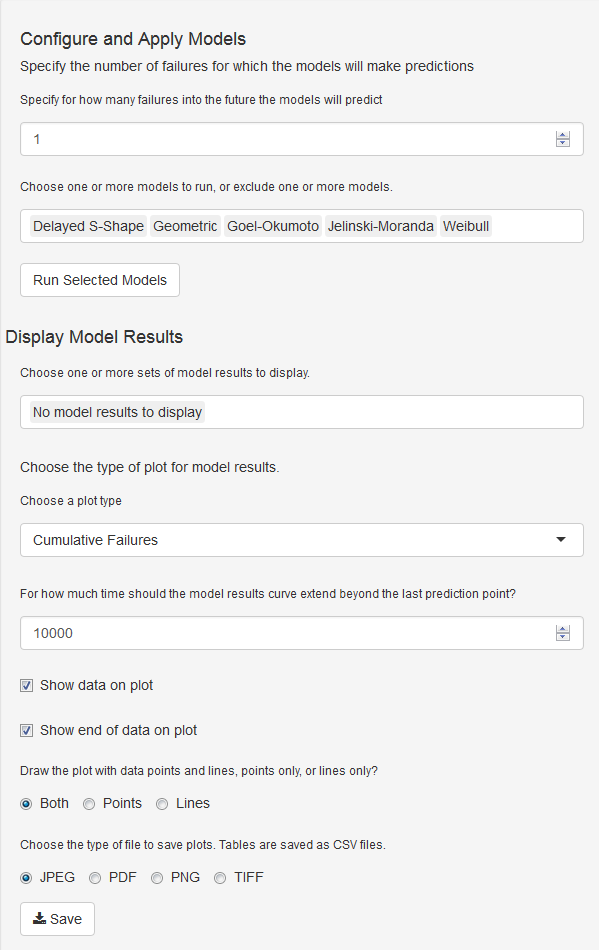
\includegraphics[width=3.4in]{Figures/Fig8}
\caption{Tab two options}
\label{fig_Tab2}
\end{figure}

Once model fitting completes, the multi-select box below ``Choose one or more sets of model results to display'' is populated with models that completed successfully. Models that fail, however, will not be available. The results of successful models can be compared against the empirical data by selecting ``Cumulative Failures'', ``Time between failures'', ``Failure intensity'', or ``Reliability growth'' from the dropdown menu below ``Choose a plot type''.

Figure~\ref{fig_SYS1_Cum} shows a plot of the observed cumulative failures along with the model fits for all five models. The solid black vertical line indicates the time at which the last failure occurred. Thus, points to the right indicate predictions. This line can be hidden by deselecting the \textbf{Show end of data on plot} checkbox. The legend at the bottom identifies the line that corresponds to each model fit. Figure~\ref{fig_SYS1_Cum} suggests that the geometric and Weibull models fit the observed data closely, whereas other models over or under predict the number of failures at various stages of testing.

\begin{figure}[!h]
\centering
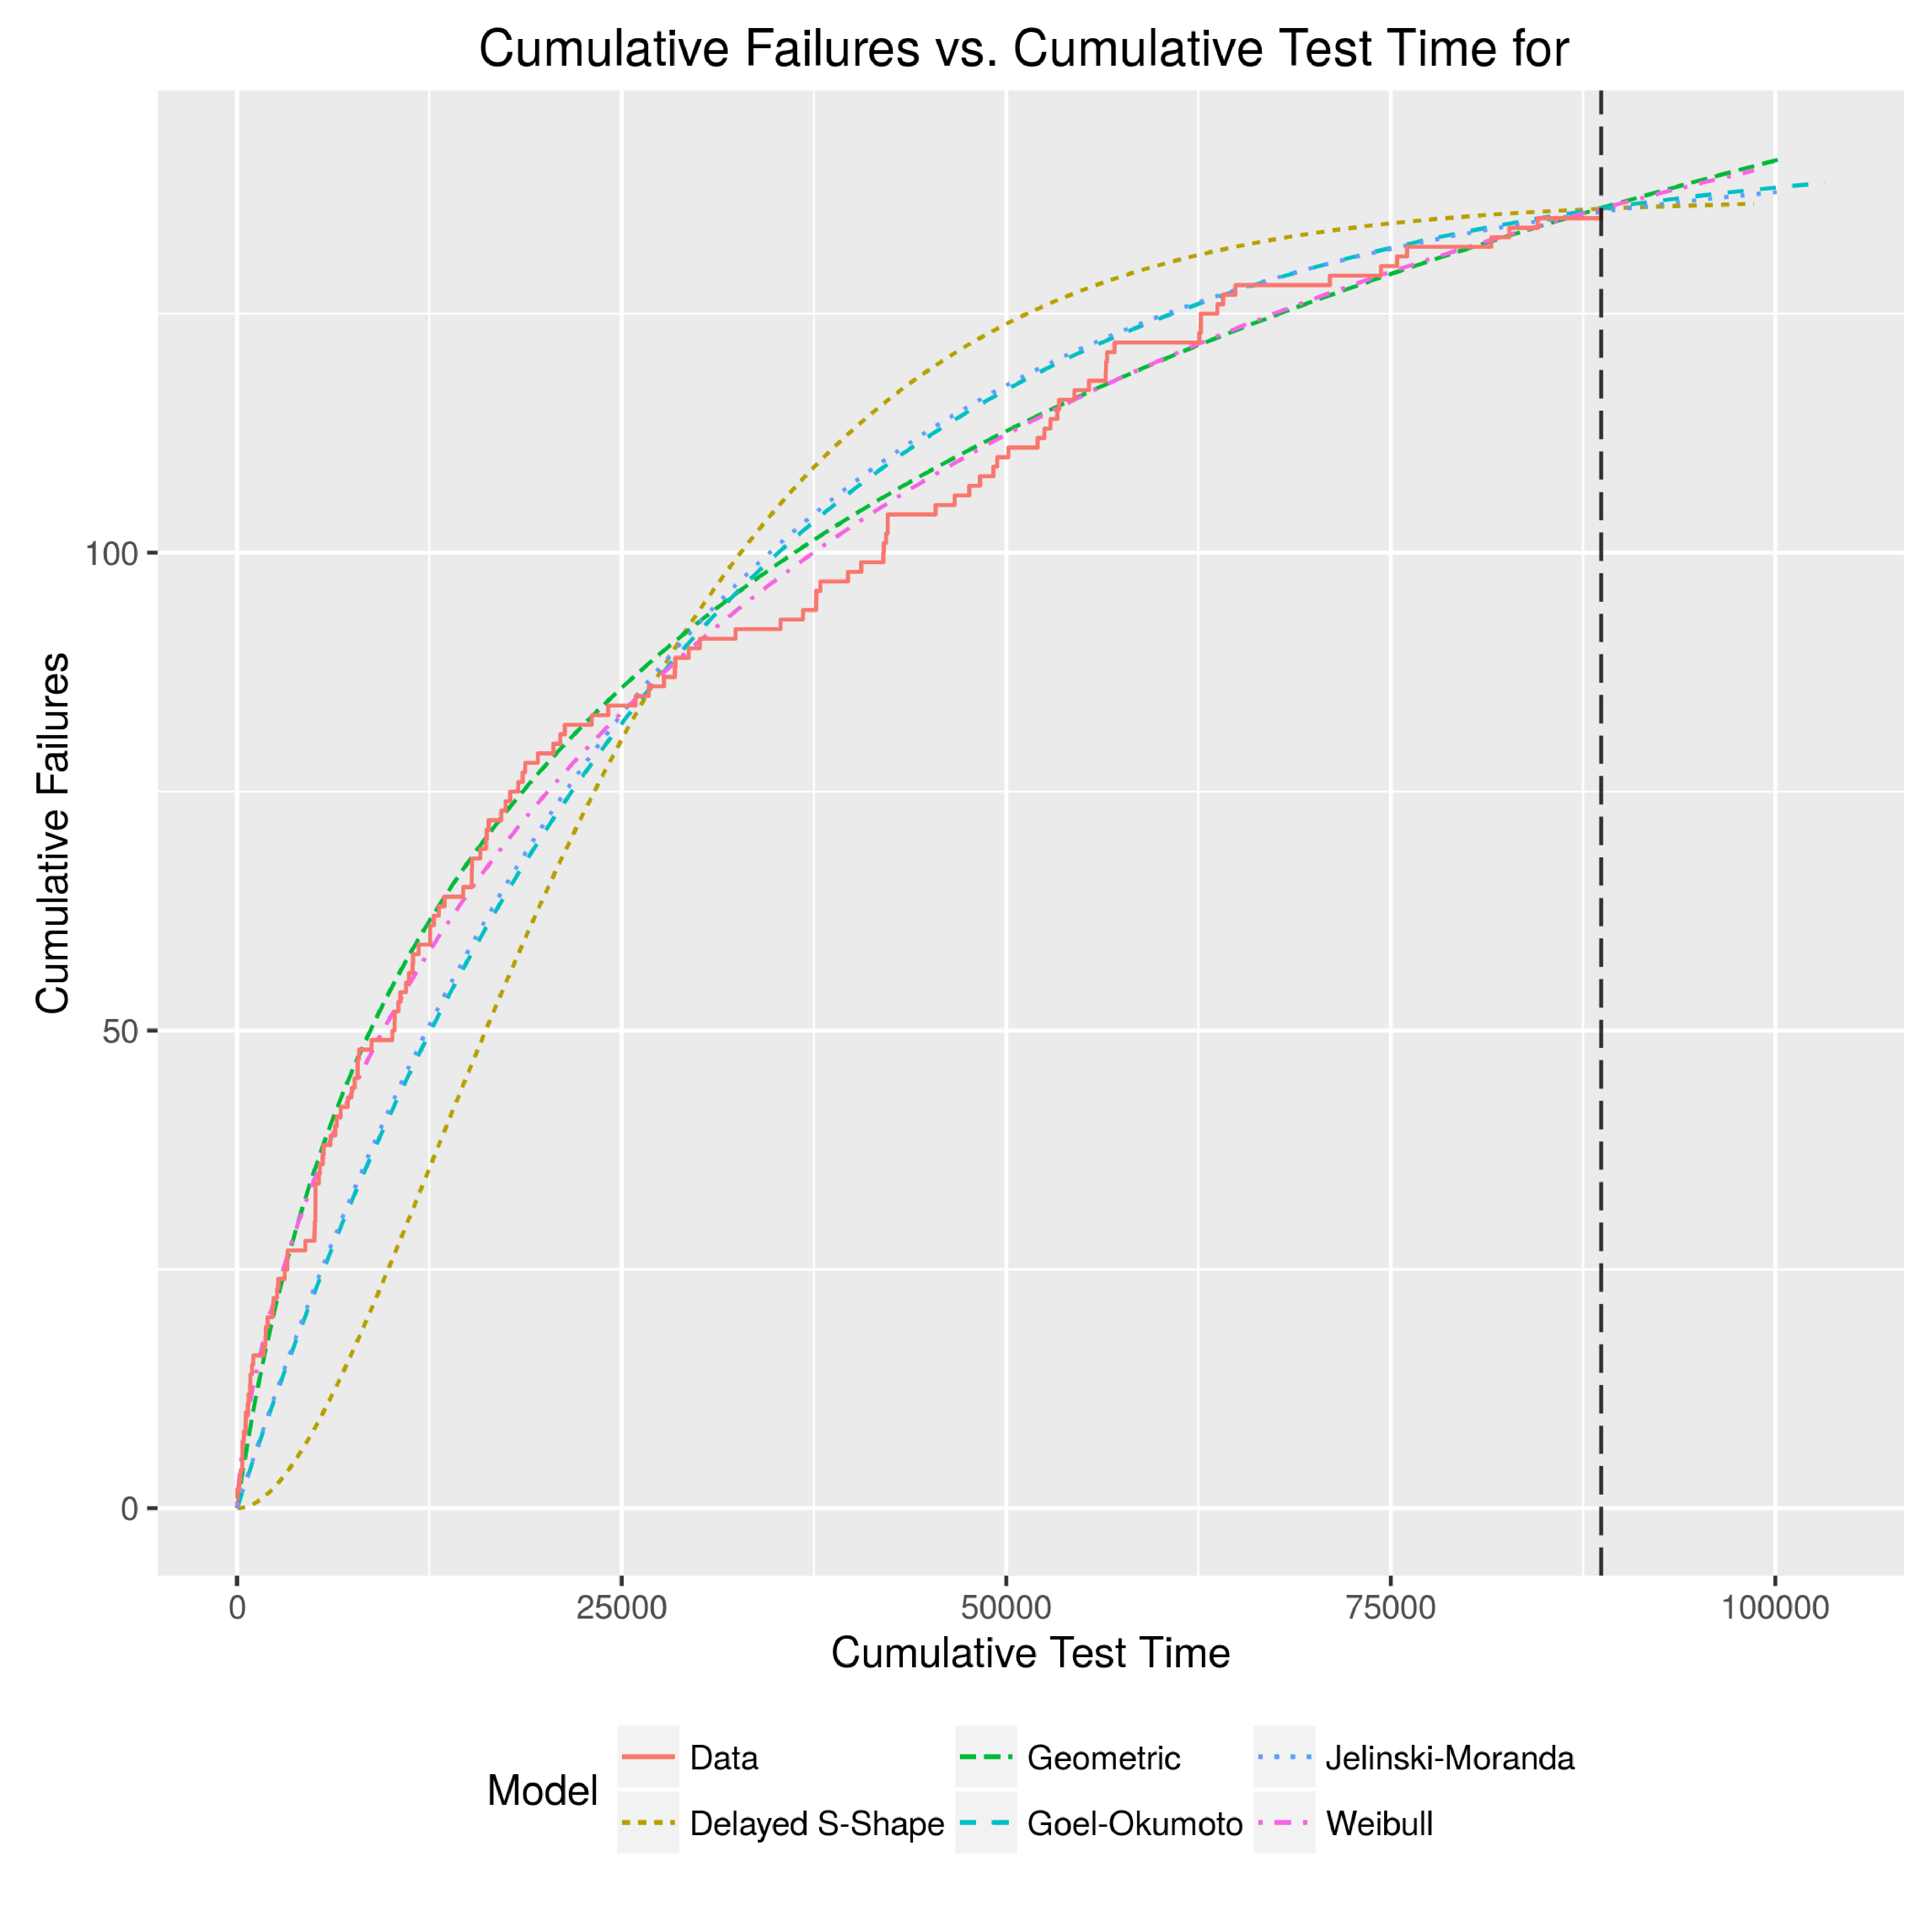
\includegraphics[width=3.4in]{Figures/SRT6}
\caption{SYS1 cumulative failures and model fits}
\label{fig_SYS1_Cum}
\end{figure}


Figures~\ref{fig_TBF},~\ref{fig_FI}, and~\ref{fig_RG} show the time between failures, failure intensity, and reliability growth data views respectively as well as with the corresponding model fits.

\begin{figure}[!h]
\centering
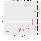
\includegraphics[width=3.4in]{Figures/TBF}
\caption{SYS1 time between failures and model fits}
\label{fig_TBF}
\end{figure}

\begin{figure}[!h]
\centering
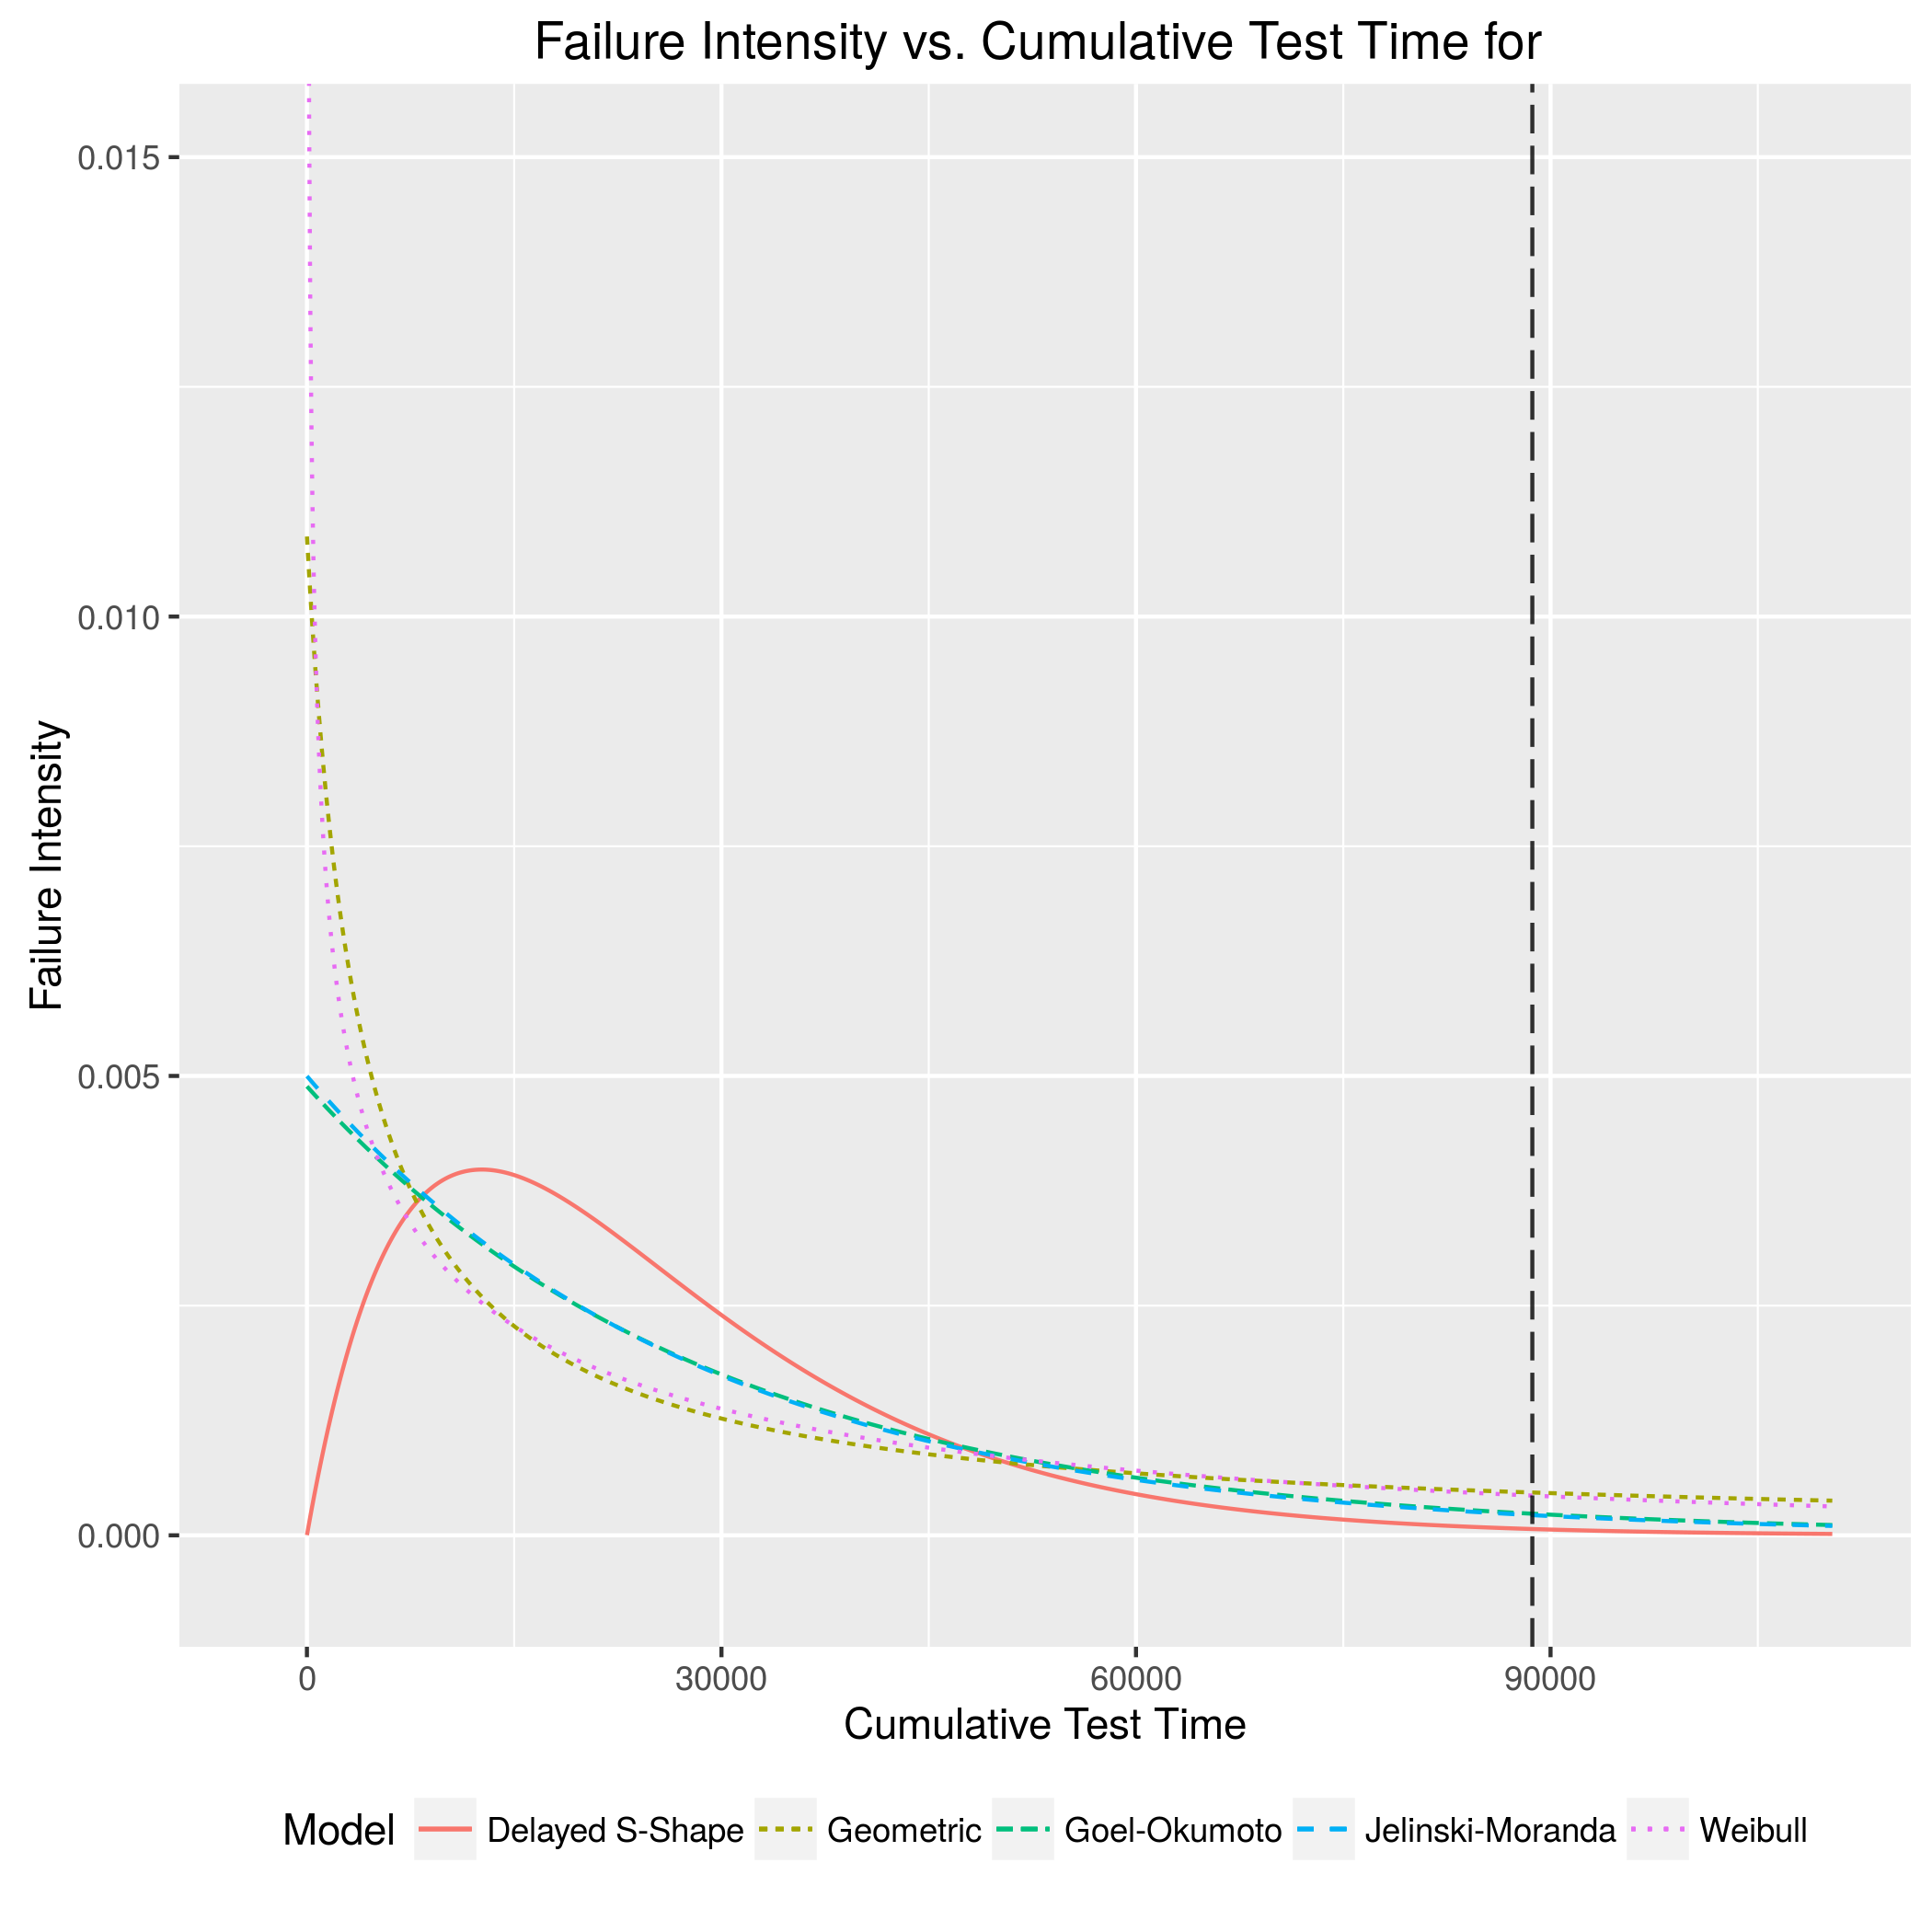
\includegraphics[width=3.4in]{Figures/FI}
\caption{SYS1 failure intensity and model fits}
\label{fig_FI}
\end{figure}

\begin{figure}[!h]
\centering
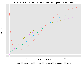
\includegraphics[width=3.4in]{Figures/Reliability_growth}
\caption{SYS1 reliability growth and model fits}
\label{fig_RG}
\end{figure}


\subsection{Tab 3: Query Model Results}\label{tab3}
Figure~\ref{fig_Tab3} shows the options on the third tab, which enable a variety of predictions. The multi-select box below ``Choose one or more sets of model results to display'' allows the user to specify a model with which they would like to make predictions. To determine the time required to observe the next $N$ failures, the user enters the number of failures in the text box below ``Specify the number of failures that are to be observed.''  Alternatively, the user may ``Specify the amount of additional time for which the software will run'' to determine the number of faults that would be detected in this interval. Entering numbers into these text boxes automatically generates a table such as Figure~\ref{fig_Tab3-table}, which shows the model names and expected number of failures for the next $t$ time units as well as the expected time required to detect the next $N$ failures. In this case, Figure~\ref{fig_Tab3-table} shows predictions for the SYS1 data set, including the time for one additional failure and the predicted number of failures to be observed in the next $100,000$ seconds of additional testing time.

\begin{figure}[!h]
\centering
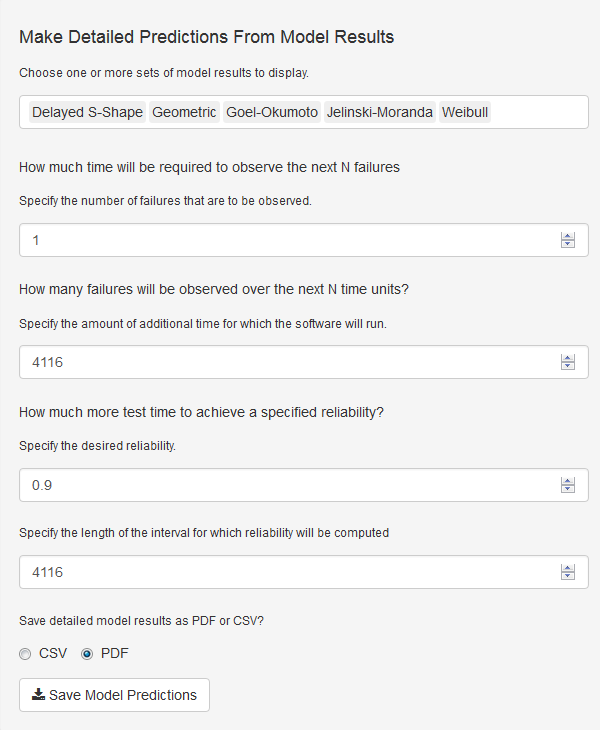
\includegraphics[width=3.4in]{Figures/Fig13}
\caption{Tab three options}
\label{fig_Tab3}
\end{figure}


\begin{figure}[!h]
\centering
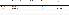
\includegraphics[width=3.4in]{Figures/Tab3-table}
\caption{Failure predictions}
\label{fig_Tab3-table}
\end{figure}


Tab three (Figure~\ref{fig_Tab3}) also provides an option to estimate the testing time required to achieve a target reliability by entering the desired reliability and time for which the software must operate without failure in the text box below ``Specify the desired reliability'' and ``How much more test time to achieve a specified reliability?'' respectively.


\subsection{Tab 4: Evaluate Models}\label{tab4}
Figure~\ref{fig_SRT_tab4} shows tab four options, which provide methods to assess model goodness of fit. The multi-select box below \textbf{Choose one or more sets of model results} allows a user to specify models they would like to apply goodness of fit measures, including the Akaike information criterion (AIC)~\cite{akaike1974new} and predictive sum of squares error (PSSE)~\cite{fiondella2011software}. The text box below ``Specify the Percent Data for PSSE'' allows specification of the fraction of data to be used to compute PSSE.

\begin{figure}[!h]
\centering
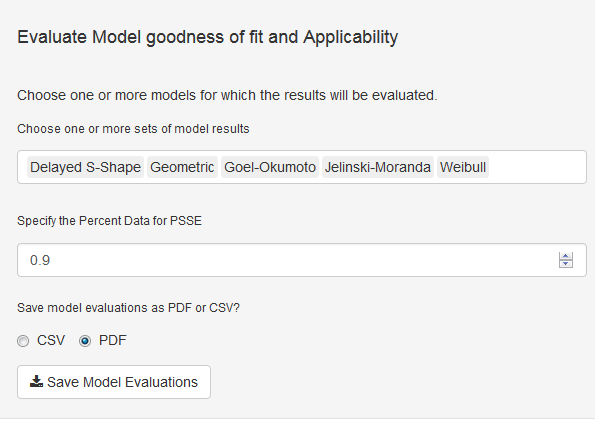
\includegraphics[width=3.4in]{Figures/Fig16}
\caption{Tab four options}
\label{fig_SRT_tab4}
\end{figure}

Figure~\ref{fig_SRT_tab4_table} shows the AIC and PSSE values for the five models applied to SYS1 when $90\%$ of data is used. The up/down arrows next to the performance measures in Figure~\ref{fig_SRT_tab4_table} sort the table based on rankings. Figure~\ref{fig_SRT_tab4_table} indicates that the Geometric and Weibull models perform best with respect to the AIC, while the Jelinski-Moranda and Goel-Okumoto models perform well with respect to PSSE.


\begin{figure}[!h]
\centering
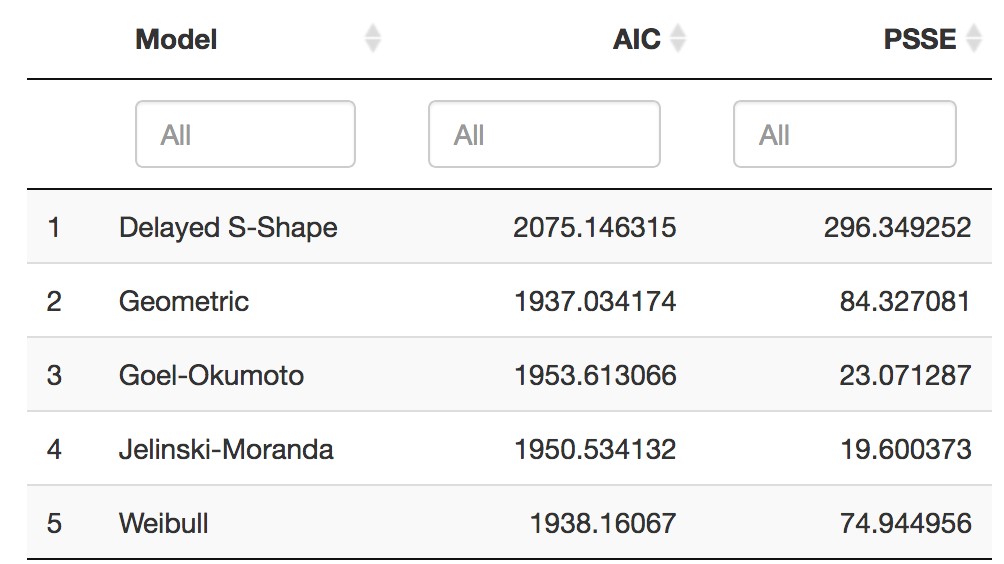
\includegraphics[width=3.4in]{Figures/SRT_tab4_table}
\caption{AIC and PSSE of all models}
\label{fig_SRT_tab4_table}
\end{figure}


\section{Automated script to generate SFRAT report}\label{sec:Script}
%This section discusses the installation and input specifications of the script.
The script is written in R programming language utilizing the Markdown library to generate the report. The script consists of $532$ lines of code including comments and blank lines between each chunk. The script consists of two files namely \textbf{report-specifications.R} and \textbf{SFRATReport.Rmd}. The \textbf{SFRATReport.Rmd} is a R Markdown file used to create reports in different formats, which contains $493$ lines of code. The \textbf{report-specifications.R} is an R script that allows the user to specify inputs necessary to run the SFRAT before generating a report, which contains $39$ lines of code.

\subsection{Installation}\label{sec:ScriptInstall}
An automated installation script is available from the GitHub repository at: https://github.com/LanceFiondella/SFRAT-Automated-Report/blob/master/installscript.R.

The manual installation procedure is:
\begin{itemize}
  \item {Make sure that your platform is either 64-bit Windows 7 or later, Mac OS X 10.9 or later, or a version of Linux capable of running R Studio.}
  \item {Perl 5 version 16 or later. Linux and Mac computers usually have this installed, however, for Windows machines Perl can be downloaded from: http://strawberryperl.com/}
  \item{Install MikTex or any other equivalent latex text editor if you are working on Windows machine.}
  \item {Install R and RStudio on your machine. You can download both RStudio and R at \textit{rstudio.com}. For Windows, Mac OS X, and Linux, you will need version R version 3.0 or later and RStudio 0.99.482 or later.
      \begin{itemize}
        \item {R (https://cran.r-project.org/) needs to be installed before RStudio can be installed. Once RStudio has been installed, the following packages need to be installed.
        \begin{itemize}
          \item {\textbf{shiny} – is a web application framework for R.}
          \item {\textbf{gdata} – is a package that provides various R programming tools for data manipulation.}
          \item {\textbf{ggplot} – is a graphical package, which offers a powerful graphics language for creating elegant and complex plots.}
          \item {\textbf{DT} – is a package that provides an R interface to the JavaScript library DataTables.}
          \item {\textbf{rootSolve} – is a package to find the roots of n nonlinear (or linear) equations.}
          \item {\textbf{knitr} – is a package that provides a general-purpose tool for dynamic report generation in R using Literate Programming techniques.}
          \item {\textbf{rmarkdown} – is a package that includes high level functions for converting R Markdown documents into a variety of formats including HTML, MS Word PDF, and Beamer.}
          \item {\textbf{markdown} - is a package for authoring HTML, PDF, and MS Word documents.}
          \item {\textbf{readxl} - is a package to import excel files.}
          \item {\textbf{formatR} - is a package designed to reformat R code to improve readability.}
        \end{itemize}
        }
        \item {You can also install the packages using the “Install packages…” menu item in RStudio’s “Tools” menu. This will bring up the dialog box as shown in Figure~\ref{fig:InstallPackages}:
        \begin{figure}[!h]
        \centering
        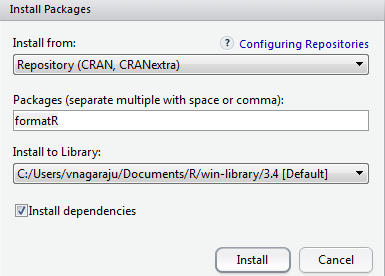
\includegraphics[width=3.4in]{Figures/InstallPackages}
        \caption{Install packages dialog box}
        \label{fig:InstallPackages}
        \end{figure}

        \noindent Specify the package(s) you want to install in the first line of the dialog box. It is not necessary to change the installation location, so just leave the second line alone. Make sure that the ``Install dependencies'' box is checked – if not, the packages you install may not work the way they should.
        }
      \end{itemize}
      }
\end{itemize}

\subsection{Script specifications}\label{sec:ScriptRun}
The user should then follow the steps described below to run the script:

\begin{itemize}
  \item {Download the contents from \textit{https://github.com/LanceFiondella/SFRAT-Automated-Report} to your desired location on your computer and unzip the folder.}
  \item {Launch R Studio and set your working directory to the location where you have saved the downloaded folder. This can be done in one of the two following ways:
  \begin{enumerate}
    \item {Go to the menu option \textbf{Session}$\to$\textbf{Set Working Directory}$\to$\textbf{To source file location} to set the working directory to the file location.}
    \item {Run the following command on the console: `setwd("/FileLocation")'.}
  \end{enumerate}
  }
  \item {Follow the steps described in Section~\ref{sec:ScriptInstall} to make sure all the required packages are installed on your machine.}
  \item {Open the file `report-specifications.R’ and specify the required input parameters that you would have specified on the SFRAT user interface:
  \begin{enumerate}
    \item {Input specifications:
    \begin{itemize}
      \item {\textbf{datapath} - Specify the path to the location where input data is saved as an excel spreadsheet. This is on Line 12.}
      \item {\textbf{sheetNumber} - If the input data file has multiple datasets arranged on different sheets, then this option allows the user to specify a particular dataset. Otherwise, specify `1' on Line 13. It is recommended to name the sheet to distinctly include the data set name in the report.}
      \item {\textbf{colors} - User can specify the colors as a list on Line 17. If nothing is specified, default set of colors will be used to display graphical results.}
    \end{itemize}
  }
    \item {Tab 1: Select, Analyze, and Filter Data
    \begin{itemize}
    \item{\textbf{confidence\_lvl} - Allows the user to specify a confidence level between $0$ and $1$ to quantify  a desired level of significance that the data exhibits reliability growth using Laplace trend test. The variable is of type `float' and can be specified on Line 20.}
    \end{itemize}
    }
    \item {Tab2: Set Up and Apply Models
    \begin{itemize}
      \item {\textbf{num\_failures\_future\_prediction} - User can specify the number of failures that they would like to predict beyond the end of testing. The number of failures should be an integer value and can be specified in Line 23.}
      \item {\textbf{models\_to\_apply} - Allows the user to specify the list of software reliability growth models that they would like to apply to make predictions. Available models are delayed s-shape (DSS), geometric (GM), Goel-Okumoto (GO), Jelinski-Moranda (JM), and Weibull (Wei) models. Model selection should be specified as a list on Line 24. }
      \item {\textbf{mission\_time} - User can specify the mission time beyond the end of testing for which they would like to see the reliability growth trend.}
    \end{itemize}
    }
    \item {Tab3: Query Model Results
    \begin{itemize}
      \item {\textbf{num\_failures\_to\_predict} - Specify the number of failures to predict beyond the end of testing. This is similar to `num\_failures\_future\_prediction' and should be specified on Line 28.}
      \item {\textbf{additional\_time\_software\_will\_run} - User can specify the additional time beyond end of testing to predict the number of failures. }
      \item {\textbf{desired\_reliability} - User can specify the target reliability between $0$ to $1$ to estimate the time required to achieve that.}
      \item {\textbf{reliability\_interval\_length}- This is to specify the mission time beyond testing to estimate the reliability.}
    \end{itemize}
    }
    \item {Tab4: Evaluate Models
    \begin{itemize}
    \item{\textbf{percent\_data\_for\_PSSE} - User can specify the percent of data to be used for model fitting. The remaining data will be used to assess model prediction capability using predictive sum of squares error (PSSE).}
    \end{itemize}
    }
  \end{enumerate}
  }

  \item{After specifying the input parameters run the following command in the console to run the script: source(‘report-specifications.R’) or you can click on ‘source’ option on the top-right corner as shown in Figure~\ref{fig:scriptsource}.
        \begin{figure}[!h]
        \centering
        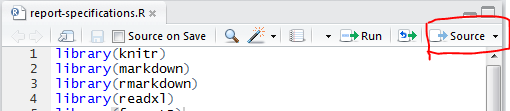
\includegraphics[width=3.2in]{Figures/scriptsource}
        \caption{Source script file}
        \label{fig:scriptsource}
        \end{figure}
  }

  \item{Upon sourcing the file, an option to display verbose is offered as shown in Figure~\ref{fig:verbose}
        \begin{figure}[!h]
        \centering
        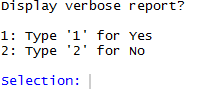
\includegraphics[width=1.8in]{Figures/verbose}
        \caption{Verbose report option}
        \label{fig:verbose}
        \end{figure}

  \noindent Select ‘1’ to display verbose report, `2' otherwise.
  }
  \item {Generated reports will be stored in the `Report' folder in the same location as the script. The file will have the following naming convention ``SFRAT report\_dataName\_YYYY-MM-DD.pdf''}
\end{itemize}


\section{Illustrations}\label{sec:Ex}
This section illustrates the use of script to analyse the failure data using SYS1 data~\cite{BookHoSRE}. The second example demonstrates the online assessment of the data using SYS1.

\subsection{Script on SYS1 data}\label{sec:Ex:Script}
This example demonstrates the use of script in the context of SYS1 data, which consists $136$ failures. 

Upon successfully installing all the required packages and downloading the script from the GitHub, open the `report-specifications.R' file using RStudio. Be sure to set the working directory to the source file location. Prepare an excel file with the input data by following the formatting requirements of the SFRAT shown in Figure~\ref{fig_Excel_sys1} and save it in your desired location. For the sake of illustration, we have taken the example data file provided in the downloaded content from GitHub. The first sheet of the `model\_data.xlsx' corresponds to the SYS1 data, which are specified below. All required inputs to all four tabs of the SFRAT tool are specified for SYS1 data as below.
\begin{lstlisting}
#Input Specifications:
#Line 12: path to the dataset
datapath <- paste0(getwd(), '/SFRAT/model_testing/model_data.xlsx')   

#Line 13: Select the sheet number in the excel file if there are multiple sheets
sheetNumber <- 1  
       
#Line 17: Specify colors for your model output
colors <- c("navy","red","green","firebrick4","magenta") 

# TAB 1: Line 20: 
confidence_lvl <- .9 #Between 0 to 1

# TAB 2: Line 23-25:
#Number of failures to predict
num_failures_future_prediction <- 2 

#Specify models to apply
models_to_apply <- c('DSS', 'GM', 'Wei','GO','JM') 

#Mission time to compute reliability growth
mission_time <- 600

# TAB 3: Line 28-31:
#Number of failures to predict
num_failures_to_predict <- 2 

#Operation/mission time
additional_time_software_will_run <- 4116 

#Target reliability between 0 to 1
desired_reliability <- .9  

#Mission time for target reliability
reliability_interval_length<- 600 

# TAB 4: Line 34: 
#Percent of data between 0 to 1 to fit models
percent_data_for_PSSE <- .9 
\end{lstlisting}

Save the `report-specifications.R' file after specifying all the required input values and click on `Source' on the top-right corner. This action will prompt a choice to select the verbose report as described in Figure~\ref{fig:verbose}. Select `1' to save a pdf of the verbose report in the folder `/Reports/SFRAT report\_SYS1\_2018-10-11.pdf'. Other formats including .docx or .html version of the document can be compiled by changing the output format in the `SFRATReport.Rmd' file on Line 6.

Figure~\ref{fig:SYS1Report} shows the initial view of the `SFRAT report\_SYS1\_2018-10-11.pdf' with a sample and description of the SYS1 data.
\begin{figure}[!ht]
\centering
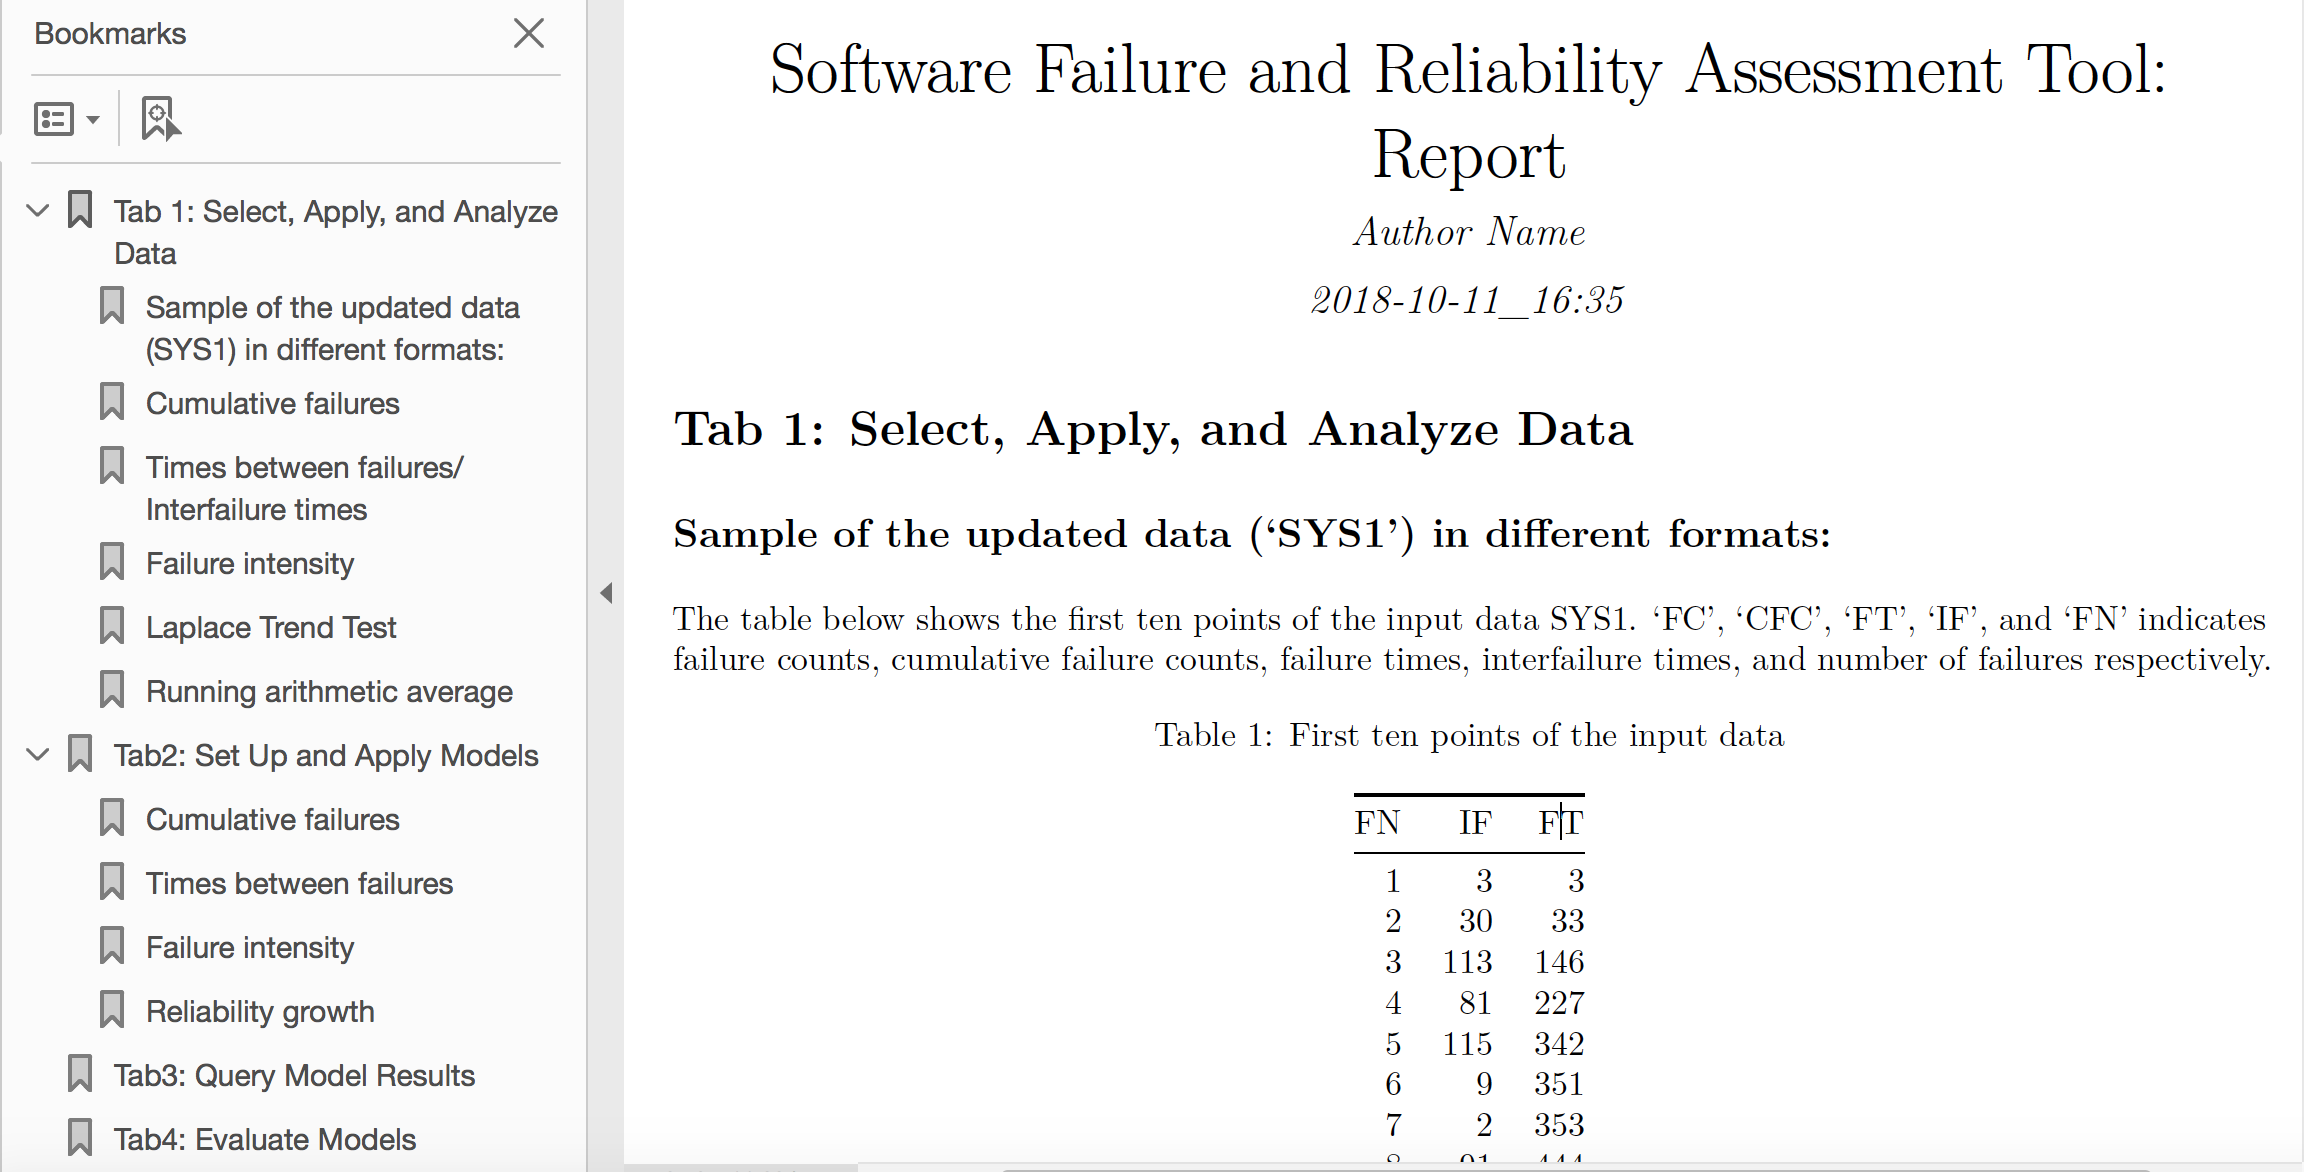
\includegraphics[width=3.4in]{Figures/SYS1Report}
\caption{Initial view of the report using SYS1 data}
\label{fig:SYS1Report}
\end{figure}

\noindent The left side of the Figure~\ref{fig:SYS1Report} shows the tab level details of all the available results in the report. The report consists of $12$ pages with each result displayed in individual page for better presentation. The Verbose report includes a brief description before the table or graph presented in each page. The first page of the report allows the user to specify the author name and change the report name as well as the date and time in the first five lines of the `SFRATReport.Rmd' file.

Figure~\ref{fig:SYS1CumFail} shows the cumulative failures of the SYS1 data with the corresponding discussion. 
\begin{figure}[!ht]
\centering
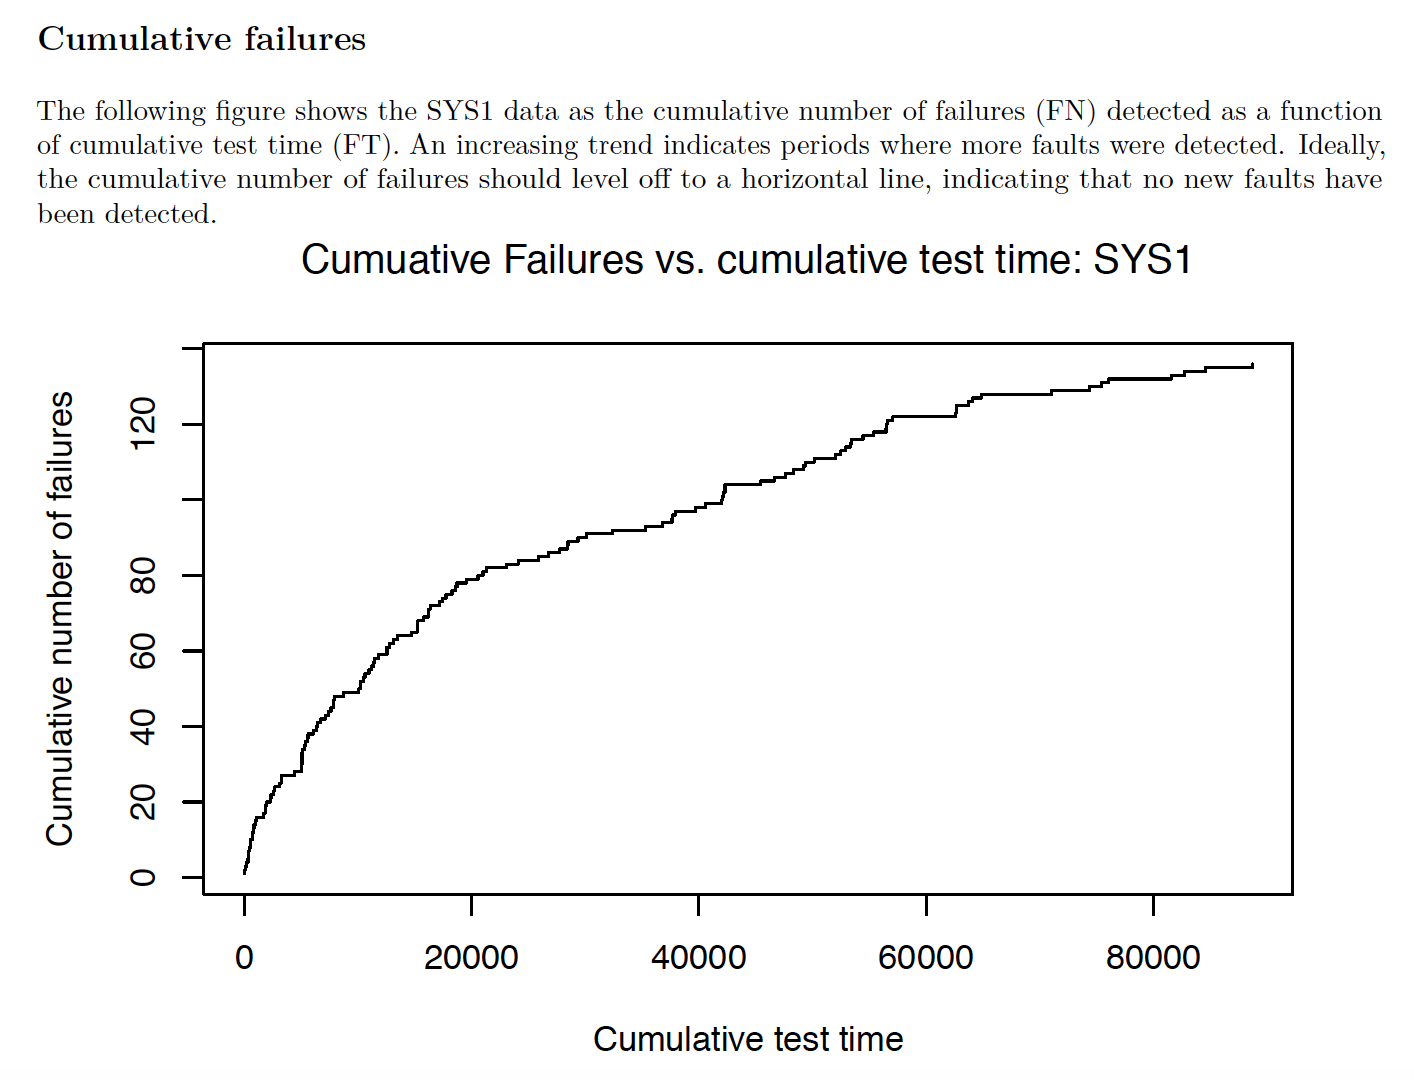
\includegraphics[width=3.4in]{Figures/SYS1CumFail}
\caption{Cumulative failures of the SYS1 data}
\label{fig:SYS1CumFail}
\end{figure}

\noindent Similar graphs for times between failures and failure intensity as a function of the testing time is displayed on Page 3 and 4 respectively.

Figure~\ref{fig:SYS1NonVerbose} shows cumulative failures of the SYS1 data as an example of the non-verbose report.
\begin{figure}[!ht]
\centering
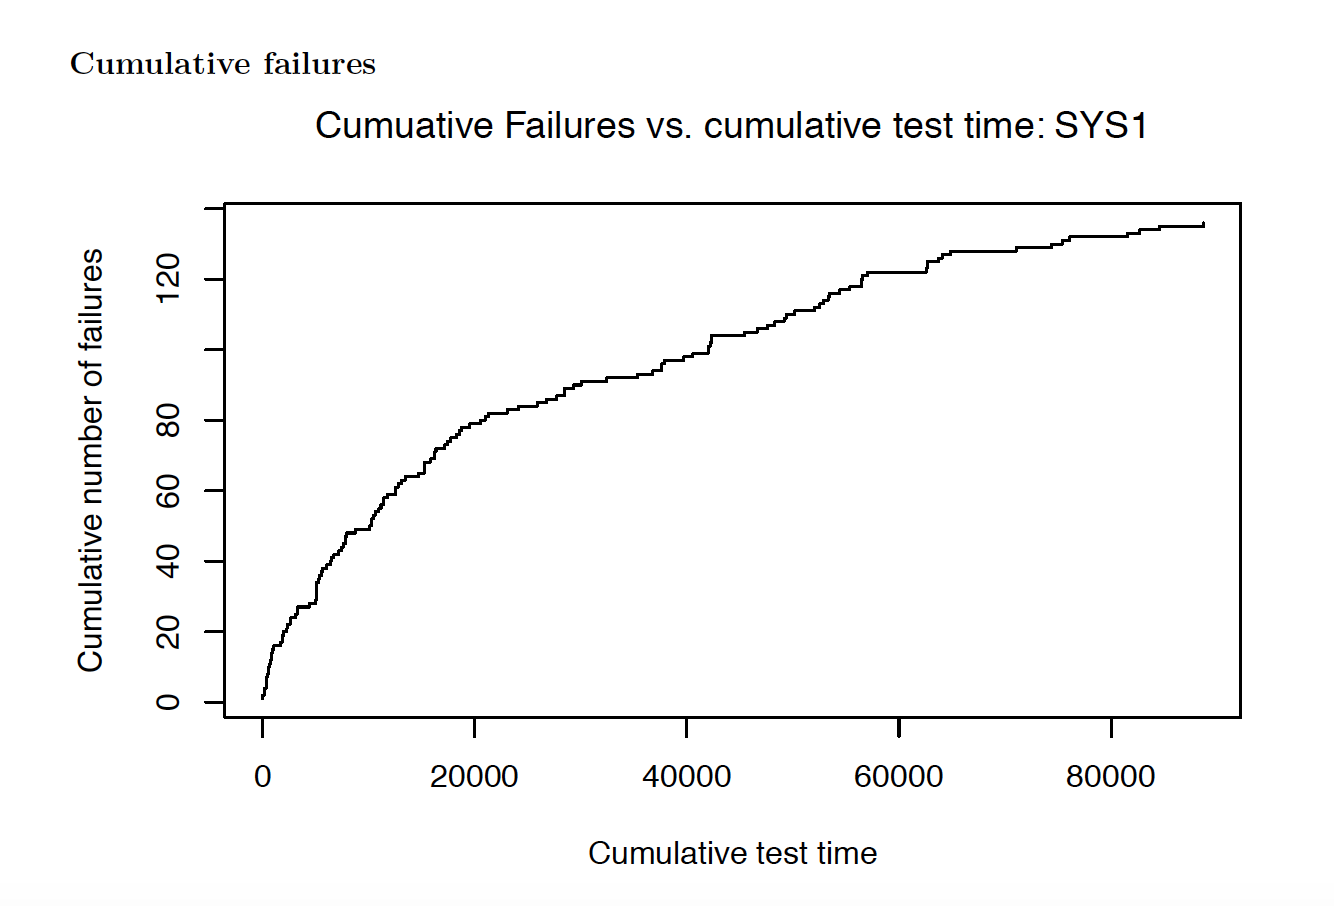
\includegraphics[width=3.4in]{Figures/SYS1NonVerbose}
\caption{Cumulative failures of the SYS1 data}
\label{fig:SYS1NonVerbose}
\end{figure}


Figure~\ref{fig:SYS1LTT} shows the Laplace trend test for SYS1 data.
\begin{figure}[!ht]
\centering
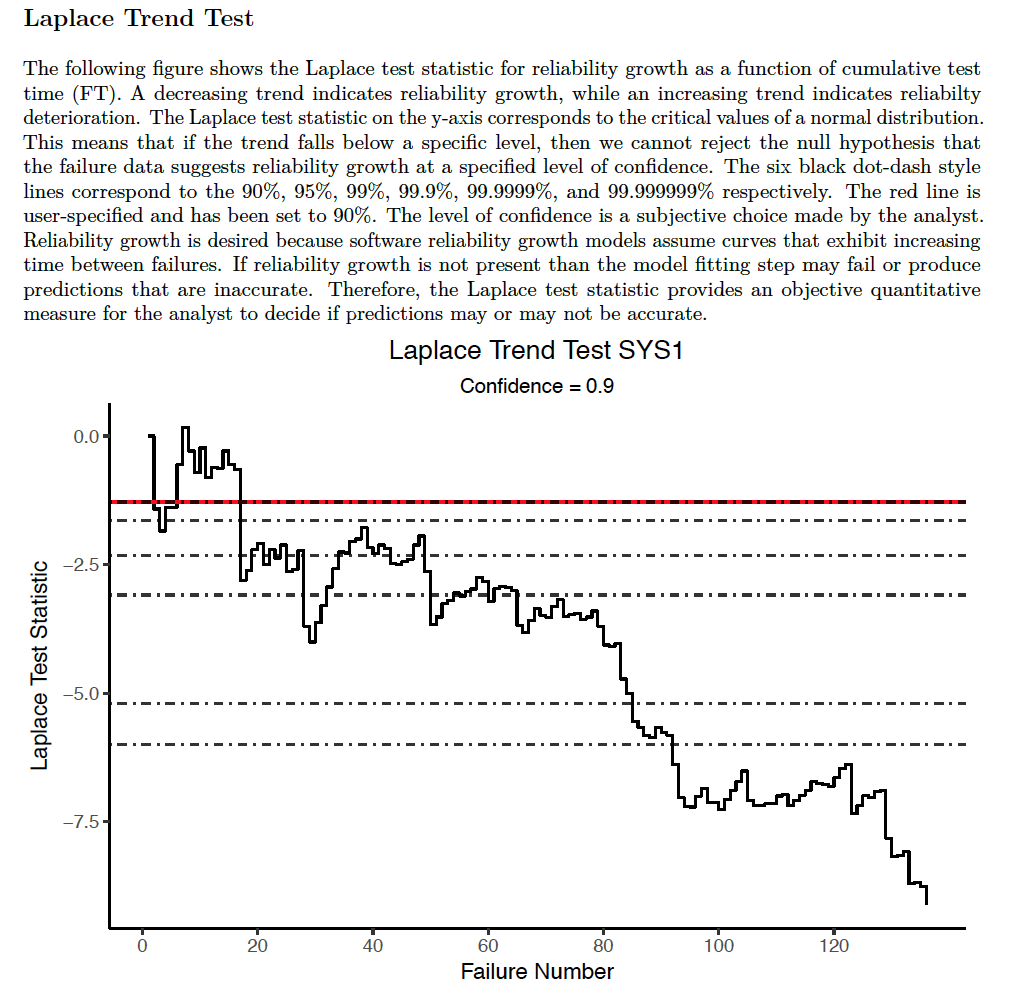
\includegraphics[width=3.4in]{Figures/SYS1LTT}
\caption{Laplace trend test of the SYS1 data}
\label{fig:SYS1LTT}
\end{figure}

\noindent Similar plot and discussion for the running arithmetic average is included in the following page in the report.


Figure~\ref{fig:SYS1Tab2} shows the first page of the Tab 2 result, which the model fit for the SYS1 data with $2$ failure predictions beyond the end of testing. The end of testing is indicated with a black vertical line.
\begin{figure}[!ht]
\centering
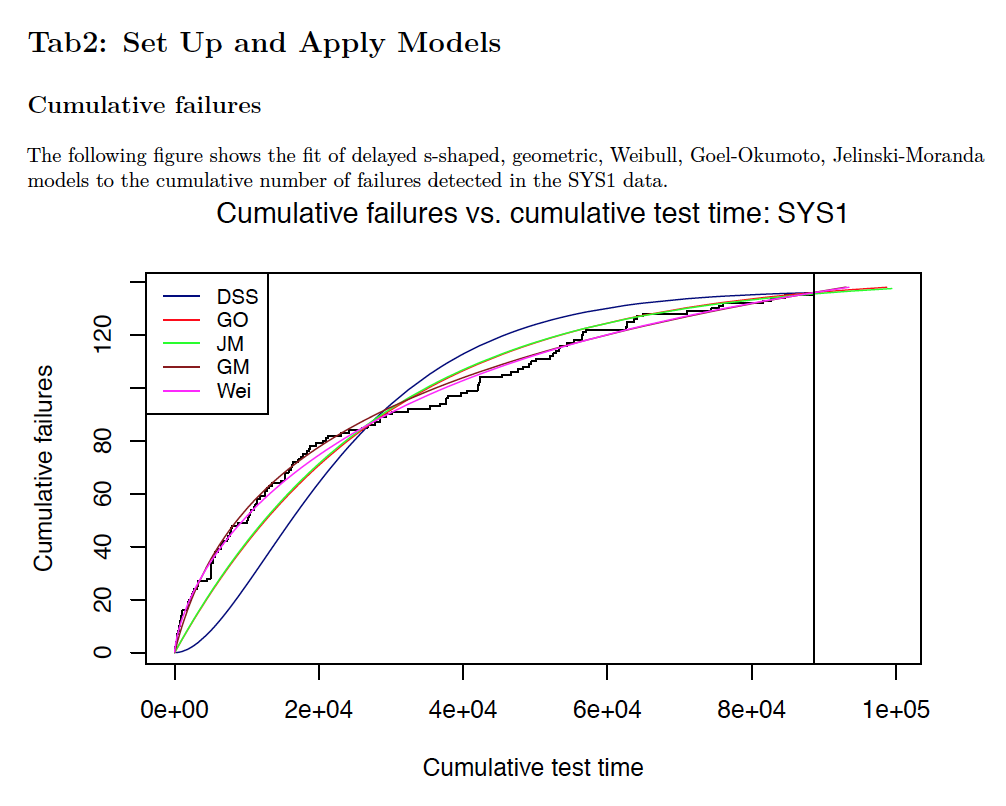
\includegraphics[width=3.4in]{Figures/SYS1Tab2}
\caption{Model fit of the SYS1 data in Tab 2}
\label{fig:SYS1Tab2}
\end{figure}

\noindent Similarly, the times between failures, failure intensity, and reliability growth for all the models are displayed between Page 8-10.


Figure~\ref{fig:SYS1Tab3} shows the predictions in Tab 3 for the selected models.
\begin{figure}[!ht]
\centering
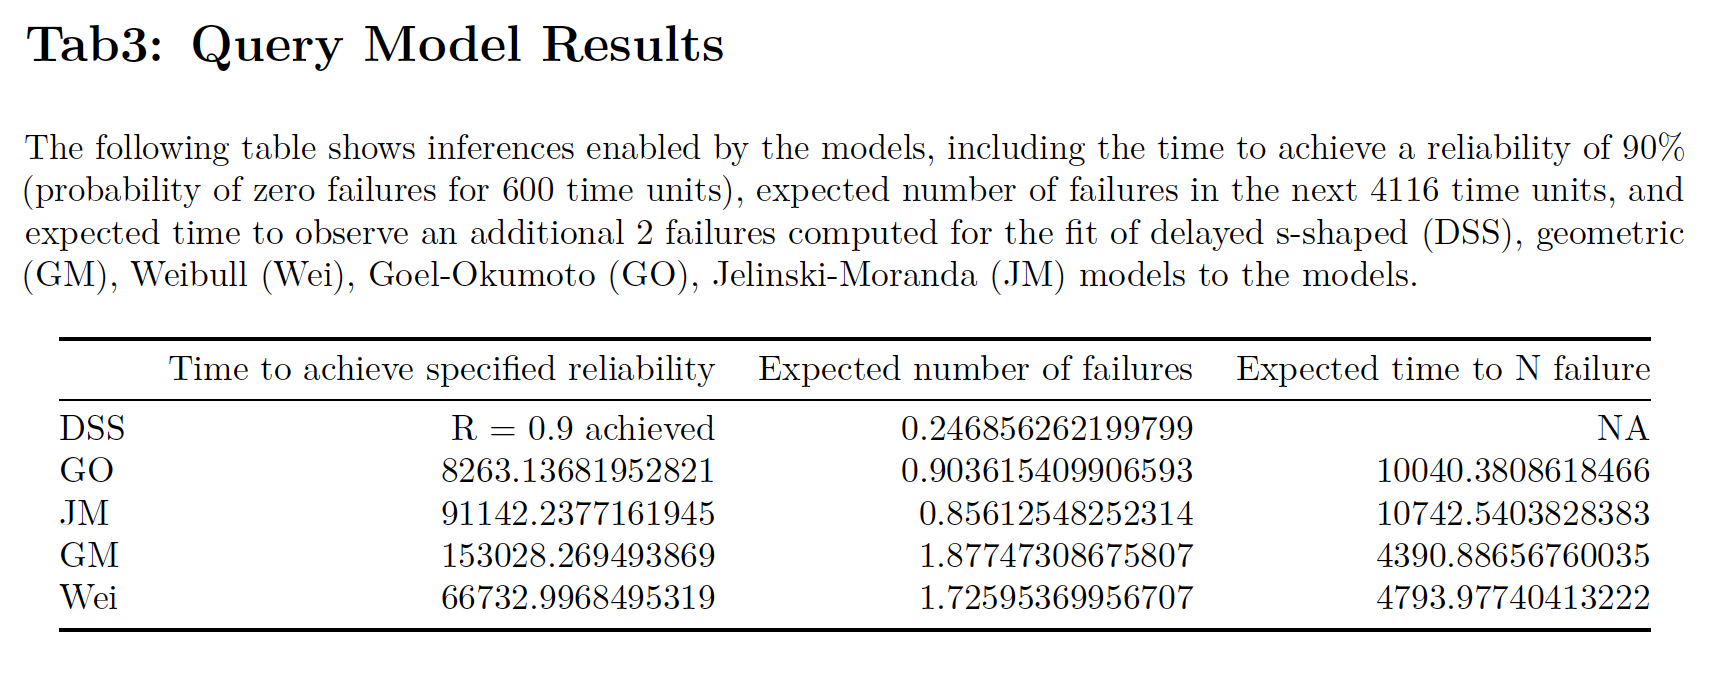
\includegraphics[width=3.4in]{Figures/SYS1Tab3}
\caption{Tab 3 results}
\label{fig:SYS1Tab3}
\end{figure}


Figure~\ref{fig:SYS1Tab4} shows the model evaluations based on the Akaike information criterion (AIC) and predictive sum of squares error (PSSE).
\begin{figure}[!ht]
\centering
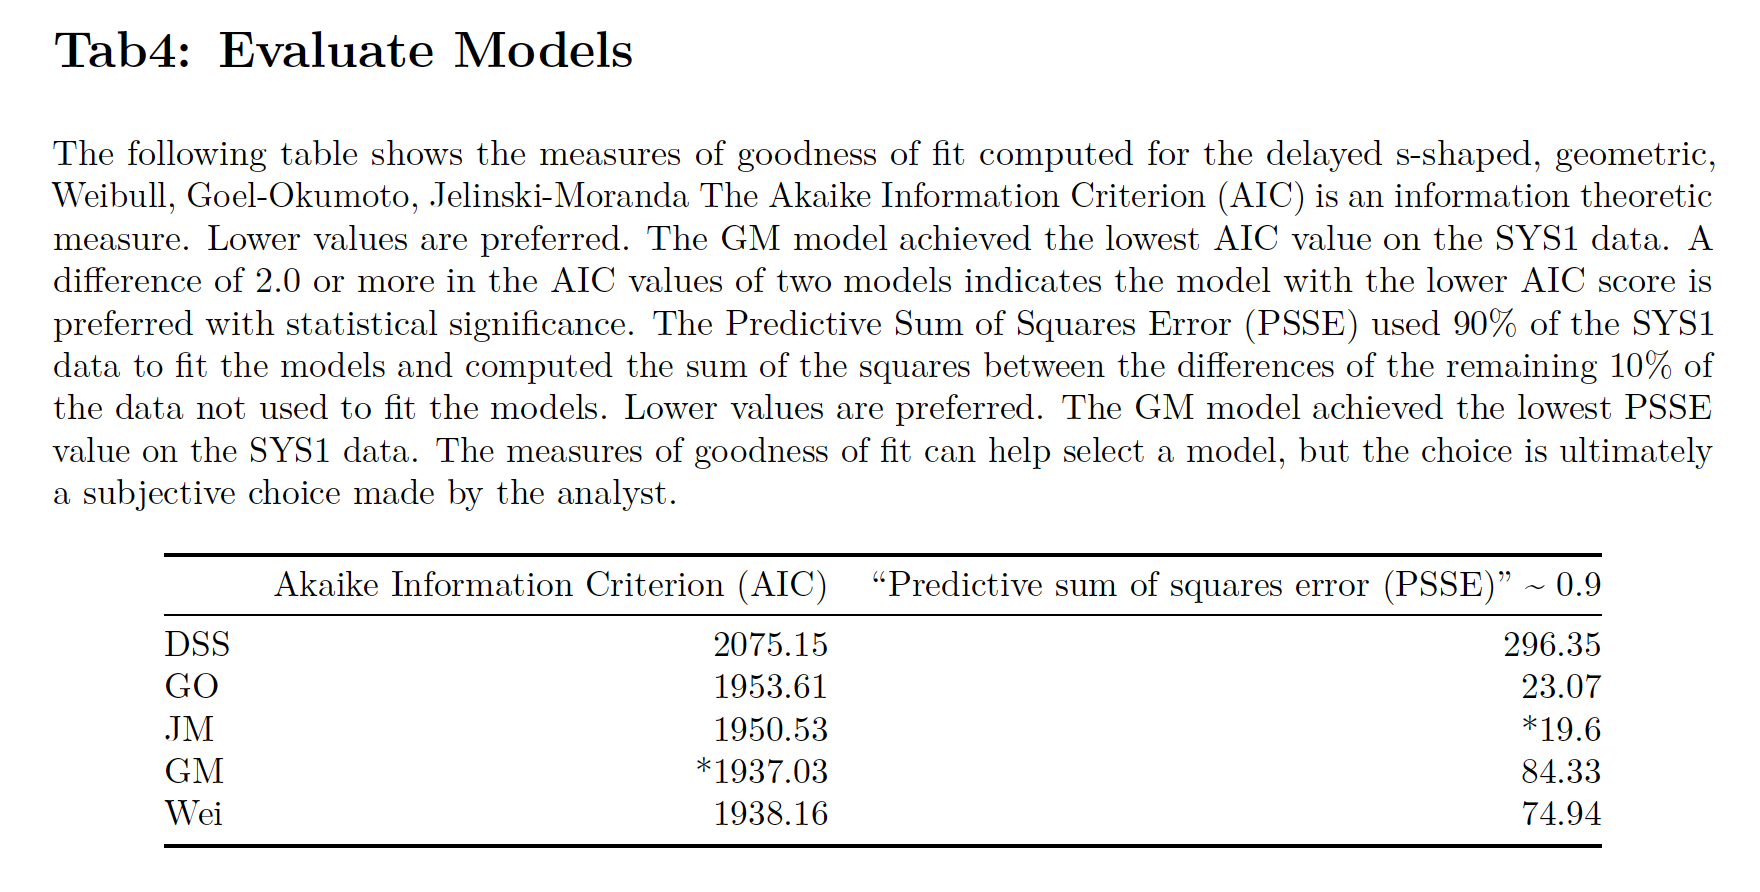
\includegraphics[width=3.4in]{Figures/SYS1Tab4}
\caption{Tab 4 results}
\label{fig:SYS1Tab4}
\end{figure}

\noindent In Figure~\ref{fig:SYS1Tab4}, the $*$ indicates the best model based on the corresponding goodness-of-fit measure.


\subsection{Online analysis using the script on SYS1 data}\label{sec:Ex:ScriptOnline}
example of application sequence that enables comparison of which model predicts best throughout the data

collection process and the assessments that might have been made if this were an ongoing activity. We can do this in the

context of sys1 and then adapt to NASA data.


\section{Conclusion and Future Work}\label{sec:Concl}
In this paper, we presented a script to automatically apply the Software Failure and Reliability Assessment Tool. An example of the SFRAT in the context of SYS1 dataset and a detailed description to run the tool is discussed. Automated pdf report generation is demonstrated using SYS1 data set. A second example is presented to illustrate the utilization of script to perform online assessment of the data. 

Future work will extend this script to accommodate the updated version of the SFRAT. The script will be ported to python programming language considering the ease of use. In addition, options to perform online data assessment will be integrated with required functionalities and measures.


\section*{Acknowledgment}\label{sec:Ack}
This work is supported by the Natioanl Aeronautics and Space Administration (NASA) SARP under Grant Number (\#). The authors would also like to acknowledge Christian Ellis, Joshua Steakelum, and Melanie Luperon for their inputs on the manuscript.


\bibliographystyle{IEEEtran}
\bibliography{bibIEEE}

\end{document}
